\documentclass[12pt,english]{article}
\setlength{\marginparwidth}{2cm}
\usepackage{todonotes}
\usepackage[utf8]{inputenc}
\usepackage[a4paper]{geometry}
\geometry{verbose,tmargin=2cm,bmargin=2cm,lmargin=2cm,rmargin=2cm}
\usepackage{color, soul}
\usepackage{amsmath}
\usepackage{tabularx}
\usepackage{layouts}
\usepackage{amsthm}
\usepackage{amssymb}
\usepackage{pdflscape}
\usepackage{pdfpages}
\usepackage{setspace}
\usepackage[authoryear]{natbib}
\usepackage[unicode=true,pdfusetitle, bookmarks=true,bookmarksnumbered=false,bookmarksopen=false, breaklinks=false,pdfborder={0 0 0},pdfborderstyle={},backref=false,colorlinks=true]{hyperref}
\hypersetup{citecolor=purple, urlcolor=green, linkcolor=red}
\usepackage{pgf,tikz,setspace,array}
\usetikzlibrary{arrows.meta}
\usepackage[official]{eurosym}
\usepackage{comment}
\onehalfspacing

\makeatletter

\setlength{\parindent}{0pt}
\setlength{\parskip}{0.5em}

%%%%%%%%%%%%%%%%%%%%%%%%%%%%%% LyX specific LaTeX commands.
\providecommand{\tabularnewline}{\\}

%%%%%%%%%%%%%%%%%%%%%%%%%%%%%% Textclass specific LaTeX commands.
\theoremstyle{plain}
\newtheorem{thm}{\protect\theoremname}
\theoremstyle{plain}
\newtheorem{prop}{\protect\propositionname}
\theoremstyle{definition}
\newtheorem{example}{\protect\examplename}
\theoremstyle{plain}
\newtheorem{lem}{\protect\lemmaname}
\theoremstyle{definition}
\newtheorem{defn}{\protect\definitionname}
\theoremstyle{plain}
\newtheorem{cor}{\protect\corollaryname}
\theoremstyle{plain}
\newtheorem{rp}{\protect\rpname}

\makeatother

\usepackage{babel}
\providecommand{\corollaryname}{Corollary}
\providecommand{\definitionname}{Definition}
\providecommand{\examplename}{Example}
\providecommand{\lemmaname}{Lemma}
\providecommand{\propositionname}{Proposition}
\providecommand{\theoremname}{Theorem}
\providecommand{\rpname}{Theorem}

\renewcommand*{\therp}{\Alph{rp}}

%%%%%%%%%%%%%%%%%%%%%%%%%%%%%% Numbered, referenceable Results.
% Usage: \resulthead{res:shortname} \textit{Statement of the result.}
% Refer to it in text as Result~\ref{res:shortname}.
\newcounter{result}
\newcommand{\resulthead}[1]{\refstepcounter{result}\label{#1}%
\noindent\textbf{Result~\theresult.}}

%%%%%%%%%%%%%%%%%%%%%%%%%%%%%%

\begin{document}
\title{Accountability and Algorithmic Delegation: Experimental Evidence}
\author{Felix B\"{o}nisch\thanks{WZB Berlin Social Science Center. Email: \texttt{boenischfelix@gmail.com}. \hl{[To do: Add acknowledgments]}}}
\maketitle

%%%%%%%%%%%%%%%%%%%%%%%%%%%%%%

\begin{abstract}
    \noindent Experimental evidence suggests that delegation can shift responsibility for adverse outcomes onto human intermediaries. We ask whether the same responsibility-avoidance motive applies to delegation to algorithms. In a preregistered online experiment with $322$ participants, a decision-maker chooses to make a payoff-relevant prediction for a matched recipient or delegate it to an algorithm, calibrated to perform equally well. We vary between subjects whether the recipient can impose punishment. The prospect of punishment reduces delegation by $18.3$ percentage points, from $60.8\%$ to $42.5\%$, reversing the direction that the responsibility-shifting account predicts. Delegation offers no protection in return. Recipients punish delegated and self-made predictions alike and condition punishment on the realized outcome. We discuss several candidate mechanisms for this reversal.
\end{abstract}
\medskip{}

\noindent \textit{JEL Classification}: C91, D91, O33

\noindent \textit{Keywords}: algorithms; delegation; responsibility; punishment; experiment

\newpage{}

%%%%%%%%%%%%%%%%%%%%%%%%%%%%%%

\section{Introduction} \label{intro}

Algorithms shape a growing share of consequential decisions. Many of these decisions carry consequences that fall, at least in part, on others. Physicians rely on diagnostic systems, firms let screening software rank job applicants, and financial advisors draw on algorithmic tools. In each setting, a human decides whether to rely on the algorithm. Who bears responsibility when the resulting decision causes harm is the subject of a lively legal \citep{lemley_remedies_2019, buiten_law_2023}, ethical \citep{matthias_responsibility_2004, santoni_de_sio_four_2021}, and policy \citep{european_commission_liability_2019,european_union_ai_act_2024} debate. Yet the normative question of where responsibility should lie is distinct from the behavioral questions of how responsibility is attributed and how those attributions shape behavior. Does delegating a decision to an algorithm change the responsibility that affected parties assign to the delegator? And does the prospect of being held responsible affect the decision to delegate? We provide experimental evidence on both questions.

For delegation between humans, the experimental literature points in a clear direction. Delegation shifts responsibility. Principals who delegate an unpopular decision to a human intermediary are punished less for it, feel less responsible for it, and delegate strategically for that reason \citep{bartling_shifting_2012, hamman_self-interest_2010, coffman_intermediation_2011, oexl_shifting_2013}. Recent evidence suggests that algorithms can inherit the intermediary's role. Delegating to an algorithm helps decision-makers escape blame for adverse outcomes \citep{feier_hiding_2022}, lets them shed moral responsibility for self-serving choices \citep{tontrup_strategic_2025} and makes dishonesty easier by obscuring intent \citep{kobis_delegation_2025}. If algorithms provide such cover, decision-makers who face potential punishment should be drawn to them, and delegation should protect the delegator when outcomes turn out badly. Yet no existing study varies whether delegators can be punished, leaving untested whether the prospect of punishment in fact motivates delegation.

We address both questions in a preregistered online experiment with 322 participants.\footnote{The preregistration (AsPredicted \#133980) is available at \url{https://aspredicted.org/hs9az8.pdf} and reproduced in full in Appendix~\ref{appendix:prereg}.} A decision-maker, Player~A, first completes ten rounds of a prediction task for her own payoff, and then makes an additional prediction that determines the payoff of a matched recipient, Player~B. Player~A can either make the consequential prediction for Player~B herself or delegate it to an algorithm calibrated to perform equally well at the task. Thus, the environment we study, a prediction task with outcome uncertainty performed by a decision-maker with no material stake in the affected party's outcome, resembles the settings in which algorithmic delegation typically operates in practice. We then vary between subjects whether Player~B can reduce Player~A's earnings. In the \textit{Punishment} condition, we elicit Player~B's punishment for every combination of delegation choice and prediction outcome, providing a within-subject test of whether delegation insulates Player~A from punishment, conditional on the outcome. In the \textit{No-Punishment} condition, no such punishment is possible. With everything except the possibility of punishment held fixed, any difference in delegation rates is attributable to that possibility, allowing us to test directly whether the prospect of being held responsible moves the delegation decision.

We find that the prospect of punishment reverses the prediction based on the literature. When punishment is possible, $42.5$ percent of decision-makers delegate to the algorithm. When it is not, $60.8$ percent do. The possibility of punishment thus \textit{reduces} delegation by $18.3$~percentage points. Delegation, in turn, offers no protection against punishment. Conditional on the outcome, Player~B punishes delegated and Player~A's own decisions similarly, and punishment responds almost entirely to the outcome of the prediction rather than to how it was made.

%old
%Thus, the possibility of punishment moves the delegation decision even though delegating draws no additional punishment. We explore several candidate explanations to reconcile these findings. A first candidate is anticipated punishment. Player~A may delegate less because she expects delegated decisions to be punished more harshly. Her elicited beliefs speak against this story. On average, her expected punishment is no higher for delegated than for self-made decisions, matching how Player~B actually punishes. A second candidate is punishment-induced effort. Facing potential punishment, Player~A may keep the decision in the hope of outperforming the algorithm. If so, non-delegators should improve on their earlier performance precisely when punishment is possible. Instead, improvement concentrates where punishment is impossible. What the data do show is selection. When punishment is possible, it is disproportionately the better-performing Player~As who keep the decision for themselves, and the delegation gap between conditions widens with performance. Both a preference for producing the good outcome oneself and a distaste for delegating uncertain decisions are consistent with this selection, but they operate in both conditions alike and cannot on their own generate the treatment difference. Lastly, not delegating can carry signaling value. By keeping the decision, Player~A may aim to convey to Player~B that she intends to try especially hard on his behalf, whereas delegating could be perceived as shirking the decision. Because the task is inherently uncertain, sending this signal requires no measurable extra effort. However, the signal carries monetary value only if Player~A expects apparent shirking to draw harsher punishment, which her beliefs do not show. Detached from actual punishment, she may instead care about Player~B's judgment itself, although this too explains the treatment difference only if the prospect of punishment is what activates this motive. Thus, while the drop in delegation under punishment is robust, which motive produces it is a question we narrow rather than settle.

The possibility of punishment thus affects the decision to delegate, even though delegating draws no differential punishment. We examine several explanations to reconcile these findings. The first is anticipated punishment. Player~A may keep the decision because she expects delegation to be punished more harshly. Her elicited beliefs provide no evidence of such an expectation and instead match how Player~B actually punishes. The second is punishment-induced effort. Player~A may keep the decision in hopes of outperforming the algorithm in the prediction task for Player~B, in which case decision-makers should improve on their earlier performance precisely when punishment is possible. Instead, improvement concentrates where punishment is impossible. Third, by keeping the decision, Player~A may aim to signal a willingness to try on Player~B’s behalf, whereas delegation may appear as shirking. Because performance is noisy, the choice to retain control can carry this signal even without a measurable improvement in performance. However, the signal carries monetary value only if Player~A expects apparent shirking to draw harsher punishment, which her beliefs do not indicate. Detached from actual punishment, Player~A may instead care directly about Player~B’s judgment. Because Player~B can form such a judgment in both conditions, however, this concern can explain the treatment difference only if the prospect of punishment activates or strengthens it. Lastly, the data show selection in performance. It is disproportionately the better-performing Player~As who retain the decision. Both an intrinsic preference for producing the good outcome oneself and a distaste for delegating uncertain decisions are consistent with this selection, but they operate in both conditions alike and cannot on their own generate the treatment difference. Thus, while the drop in delegation under punishment is robust, which motive produces it is a question we narrow down rather than settle.

%The possibility of punishment thus moves the delegation decision even though delegating draws no additional punishment. We examine several explanations to reconcile these findings. The first is anticipated punishment. Player~A may keep the decision because she expects delegation to be punished more harshly. Her elicited beliefs show no such expectation, and instead match how Player~B actually punishes. The second is punishment-induced effort. Player~A may keep the decision in the hope of outperforming the algorithm in the prediction task for Player~B, in which case decision-makers should improve on their earlier performance precisely when punishment is possible. Instead, improvement concentrates where punishment is impossible. What the data do show is selection. It is disproportionately the better-performing Player~As who keep the decision, and the delegation gap between conditions slightly widens with performance. Both an intrinsic preference for producing the good outcome oneself and a distaste for delegating uncertain decisions are consistent with this selection, but they operate in both conditions alike and cannot on their own generate the treatment difference. Lastly, by keeping the decision, Player~A may aim to merely convey to Player~B that she intends to try especially hard on his behalf, whereas delegating could be perceived as shirking the decision. Because the task is inherently uncertain, sending this signal requires no measurable additional effort. However, the signal carries monetary value only if Player~A expects apparent shirking to draw harsher punishment, which her beliefs do not show. Detached from actual punishment, she may instead care about Player~B's judgment itself, although this too explains the treatment difference only if the prospect of punishment is what activates this motive. Thus, while the drop in delegation under punishment is robust, which motive produces it is a question we narrow rather than settle.

Our contribution is twofold. First, we provide, to our knowledge, the first direct test of whether the prospect of punishment encourages delegation to an algorithm, as prior evidence on delegation to human intermediaries would predict \citep{bartling_shifting_2012, hamman_self-interest_2010, coffman_intermediation_2011, oexl_shifting_2013}. Our environment departs from these canonical designs in three respects. The intermediary is an algorithm rather than a person. The decision involves genuine uncertainty, so a bad outcome may reflect bad luck rather than bad intent. And its immediate consequences fall entirely on the recipient, so the underlying decision involves no tradeoff between the players’ payoffs and there is no self-serving choice to police. In this environment, the effect runs in the opposite direction. The prospect of punishment discourages rather than encourages delegation, and it does so selectively among the decision-makers most likely to succeed. This reversal is the paper's main empirical result, adding a determinant of preferences over algorithm use that operates through the decision context rather than through algorithm characteristics or the task.

Second, we use Player~B's punsihment decision to examine how an affected party assigns responsibility for algorithmic delegation when the delegation choice is uninformative about relative ability. The closest precedent is \citet{feier_hiding_2022}, whose treatments vary whether the intermediary is an algorithm or another participant under a fixed punishment regime, whereas we hold the intermediary fixed as an algorithm and vary whether punishment is possible. In their environment, decisions delegated to an algorithm are rewarded more generously than non-delegated decisions after bad outcomes. However, the same subject both makes a delegation choice and evaluates the decision, so that evaluations may partly reflect participants’ own delegation choices. Moreover, the delegation decision is strongly determined by beliefs about relative ability between oneself and the intermediary, inviting punishment of overconfidence rather than of delegation itself. Our design is intended to remove both channels by separating the delegator and evaluator roles and making delegation uninformative about relative ability. Once both channels are closed, the differential disappears, and punishment tracks the realized outcome instead.

The remainder of the paper is organized as follows. Section~\ref{literature} relates the study to the literature. Section~\ref{design} presents the experimental design and hypotheses. Section~\ref{results} reports the results and examines candidate mechanisms. Section~\ref{conclusion} concludes.

%Three design features distinguish our setting from the closest precedent, \citet{feier_hiding_2022}, two of them central to identification. First, the algorithm is calibrated at the \textit{individual} level rather than the session or group level. Existing designs typically expose subjects to a distribution of algorithmic performance and let them infer their own ability relative to that distribution; the delegation decision then carries strong signal value about the principal's self-perception, and any differential punishment can reflect overconfidence rather than responsibility shifting per se. By neutralizing relative-performance signaling at the individual level, we isolate the responsibility-shifting motive. Second, our \textit{No-Punishment} condition turns off the punishment possibility entirely, allowing us to identify the effect of anticipated punishment on the delegation decision itself---a test that none of the existing algorithmic-delegation designs permits. Third, we separate the delegator and evaluator roles across disjoint subject pools, rather than having the same subjects play both, removing the self-justification motives that a dual role can introduce into the punishment decision. Together these features sharpen the test of responsibility shifting in algorithmic delegation that the literature has thus far been able to deliver.

%These findings contribute to three strands of literature. First, we add to the experimental literature on responsibility avoidance through delegation \citep{bartling_shifting_2012,coffman_intermediation_2011,oexl_shifting_2013,hamman_self-interest_2010,hill_does_2015,steffel_passing_2016}, by extending the canonical setting to delegation to an algorithmic intermediary in a setting with genuine outcome uncertainty. Second, we contribute to the rapidly growing literature on algorithm aversion and adoption \citep{dietvorst_algorithm_2015,logg_algorithm_2019,burton_systematic_2020,mahmud_what_2022,chugunova_we_2022} by isolating an under-studied determinant of algorithm use: the institutional context in which the human user is held accountable. Third, and most directly, we build on \citet{feier_hiding_2022} and \citet{kirchkamp_sharing_2019} by providing a clean experimental test of two long-standing claims in the responsibility-and-algorithms literature, with a design that controls relative-performance signaling at the individual level and that includes a condition in which punishment is ruled out by construction. The contrast with \citet{feier_hiding_2022} is consequential: that study finds that decision-makers are held \textit{less} responsible for algorithmically delegated decisions, while we find that the punishment possibility \textit{reduces} delegation rather than increasing it. We argue that the two findings are reconcilable: the relative-performance signaling that drives much of Feier et al.'s differential punishment is closed off by construction in our design, isolating a different and milder margin (the motivational salience of accountability for the principal). Beyond the experimental literature, our findings speak to the regulatory debate over the assignment of responsibility for algorithmic decisions \citep{european_union_ai_act_2024}: within the bounds of the setting we study, holding human users accountable for algorithm-mediated outcomes appears to be a behavioral lever for direct human engagement with the decision, rather than merely a tool for ex-post moral attribution. We are explicit in Section~\ref{conclusion} about why the present evidence---a single online experiment on a stylised prediction task with one UK Prolific sample---supports this claim only in a bounded sense, and what would be required to extend it to the high-stakes algorithmic domains (medical, judicial, hiring, financial) that motivate the regulatory debate.


\section{Related Literature} \label{literature}

%This paper bridges three strands of literature: (i) responsibility avoidance through delegation, an established line of experimental work in which the intermediary is another human; (ii) algorithm use, which examines when and why people are willing to use algorithmic decision aids, for themselves and others; and (iii) responsibility attributions to decisions involving algorithms, an emerging literature at the intersection of the first two.

%[Comment: Is this first paragraph really necessary? Is it perhaps better placed in a conclusionary paragraph of the whole literature section, perhaps introducing the summary of the contribution of the paper (e.g. in the intro)?]

\subsection*{Responsibility avoidance through delegation}

Delegation has long been studied as an efficiency-enhancing institutional arrangement: principals delegate to agents who have better information, lower opportunity costs, or specialised skills. Alongside these efficiency motives, a separate literature has identified a range of strategic motives for delegation, e.g. as a commitment device that alters the equilibrium (Fershtman and Gneezy, 2001), as a way to motivate the agent (Aghion and Tirole, 1997), or as a means of shifting responsibility for the outcome away from the principal, i.e. principals may delegate not because the agent is more competent or cheaper, but because doing so shifts responsibility for the resulting outcome away from themselves --- both in their own eyes (felt responsibility for the outcome) and in the eyes of others (the blame others attribute to them). The political-science and public-choice literatures have long recognized that delegation can serve as a strategy for shifting blame onto an intermediary~\citep{weaver_politics_1986, fiorina_legislator_1986}. Experimental economics has established the same motive in incentivised settings, primarily using modified dictator games.

\citet{bartling_shifting_2012} provide the canonical experimental evidence. In their design, a dictator may either choose between a fair and an unfair allocation of an endowment or instead delegate this choice to another person whose monetary incentives are aligned with the dictator's. The recipient is adversely affected if the unfair allocation is chosen and may punish the dictator and the intermediary. They find that through delegation punishment is effectively shifted from the dictator to the intermediary, and the prospect of avoiding punishment constitutes a strong motive for the delegation decision itself. \citet{coffman_intermediation_2011} reinterprets the mechanism behind this punishment reduction. He finds that the principal can no longer avoid punishment when she directly interacts with the receiver despite the intermediary's presence, suggesting that what reduces punishment is the absence of direct interaction with the affected party rather than any transfer of blame to a deciding intermediary. This holds even when the intermediary remains completely passive. \citet{oexl_shifting_2013} sharpen this reading by modifying the canonical game so that delegation necessarily eliminates the fair option. The principal nevertheless escapes punishment, with the intermediary actively choosing between two unfair allocations after delegation. Finally, both \citet{bartling_shifting_2012} (with a die roll) and \citet{oexl_shifting_2013} (with an intermediary-triggered random draw) include treatments that substitute a randomization device for the human intermediary. In both, the principal still shifts some punishment to the device, though less than under delegation to a deciding human. Across the two papers, two distinct components of the responsibility-shifting effect emerge --- the absence of direct interaction between principal and recipient drives the reduction in principal punishment, while the act of choosing, rather than any contribution to outcome unfairness, is what transfers blame to the intermediary.

The motive is not confined to settings with third-party punishment.  \citet{hamman_self-interest_2010} extend this picture in a setting without third-party punishment. Still, principals' transfers to recipients fall sharply when they delegate, indicating that responsibility-shifting can operate through felt responsibility or moral wiggle room rather than through the avoidance of punishment. Qualitative self-reported responsibility and recipient-side blame attributions are consistent with this reading---dictators feel less responsible when they delegate, and recipients place less blame on principals than on intermediaries.

%Lastly, \citet{argenton_potters_yang_2023} document the mirror pattern on the credit side: delegators receive less credit for fair outcomes when they delegate than when they choose directly, so that the responsibility-attribution structure operates symmetrically across blame and credit---though magnitudes are not.

Beyond the canonical dictator-game setting, the responsibility-shifting motive --- and the strategic use of delegation it gives rise to --- has been documented across a range of domains. In incentivised ultimatum bargaining, proposers using a hired delegate extract larger surpluses \citep{fershtman_gneezy_2001}. In sequential voting, non-pivotal voters are punished less than pivotal ones for the same group outcome and voters strategically vote against their preferred allocation to avoid being pivotal \citep{bartling_fischbacher_schudy_2015}. For acts of deception, principals pay an agent to lie on their behalf \citep{erat_avoiding_2013}. In policy-making, observers rate delegating legislatures as less blameworthy than legislatures who decide directly, even when the delegate is powerless to change the outcome \citep{hill_does_2015}. \citet{freer_friedman_weidenholzer_2024} isolate the motive in financial decision-making, finding that a substantial fraction of investors delegate even purely luck-based lottery choices, where alternative motives --- decision costs, performance-chasing, or risk tolerance --- cannot rationalize the choice. 

%\citet{steffel_passing_2016} show that people are more willing to delegate decisions made on behalf of others than decisions made for themselves, especially when those decisions might have negative outcomes. Thus, people seem to care more about avoiding blame for bad outcomes than about claiming credit for good ones. [Comment: Perhaps this can be left out here, because we come back to it in the results section?]

In sum, the canonical literature documents that in settings with self-interested choice, delegation reduces principal punishment and her felt responsibility, in turn motivating delegation. Our setting departs from this canonical design along three dimensions: the intermediary is algorithmic rather than human, the outcome falls entirely on a third party rather than partly on the principal herself, and the underlying decision involves genuine predictive uncertainty rather than a known fair/unfair choice. Whether the responsibility-shifting motive retains its force under these conditions is the question we take up.

\subsection*{Delegation to algorithms}
A large and rapidly growing empirical literature studies when and why people are willing to use algorithmic decision aids, beginning with \citet{dietvorst_algorithm_2015}, who introduce the term \textit{algorithm aversion} --- the finding that people prefer their own (or other humans') judgement over algorithmic predictions, even after observing that algorithms outperform human decision-makers. In contrast, \citet{logg_algorithm_2019} document conditions under which subjects show \textit{appreciation} of algorithmic advice over human advice; the picture that emerges is therefore one of substantial heterogeneity in algorithm preferences across tasks, contexts, and elicitation methods. \citet{burton_systematic_2020}, \citet{mahmud_what_2022}, \citet{chugunova_we_2022}, and \citet{qin_ai_2025} provide systematic reviews of this literature and document a large array of moderators for when and why algorithms are used in decision-making. For example, algorithm aversion is stronger when the algorithm cannot be observed to learn from its mistakes \citep{berger_watch_2021}, when the algorithm's reasoning is opaque \citep{litterscheidt_financial_2020,sharan_dont_2020}, and when the algorithm is presented as more complex \citep{stein_dont_2020}. Algorithm aversion is also stronger when the task is perceived as more uncertain \citep{dietvorst_people_2020}, when delegation removes any ability to override the algorithm's choice \citep{dietvorst_overcoming_2018}, and when the algorithm is used in tasks perceived as subjective \citep{castelo_task-dependent_2019,bogert_humans_2021}. Recent additions include \citet{bockstedt_humans_2025}, who show that loss-framing of decision tasks eliminates the preference for human assistance over AI assistance, and \citet{ivanova_stenzel_measuring_2024}, who develop a menu-based design to elicit willingness to cede control to algorithms versus humans.

[Comment:
- the literature reviews and references in general are old-ish...ideally we can include more recent references.
- Maybe include the Dargies, Hakimov, Kübler reference here.
- Also think about where to include the two ivanova stenzel papers]

\subsection*{Responsibility perceptions of decisions involving algorithms}
Within this body of work, a smaller subset focuses on algorithm-use preferences in settings whose consequences fall partly or wholly on someone other than the decision-maker, sometimes called the \textit{moral domain}. The consensus is that aversion to algorithms is amplified once third-party welfare is at stake. \citet{gogoll_rage_2018} document this in an incentivised calculation task with performance uncertainty (both humans and the algorithm can err), \citet{bigman_people_2018} in vignettes across high-stakes moral domains (driving, legal, medical, military); and \citet{jauernig_people_2022} in an incentivised allocation task that identifies \textit{moral discretion} as the human capacity people specifically value.

Once decisions affect a third party, the responsibility-shifting motive established for human delegation becomes relevant for algorithmic delegation as well.

A first strand of evidence, predominantly vignette-based and unincentivised, examines how third parties attribute responsibility and blame to human actors involved with algorithms. In the medical domain, \citet{pezzo_pezzo_physician_2006} document the same pattern for a doctor who follows a (bad) recommendation from an automated decision aid, and \citet{tobia_when_2021} extend the discussion to liability law: physicians who follow standard-care AI recommendations face reduced legal exposure --- and the authors argue that this constitutes an incentive to follow such recommendations specifically because doing so shields physicians from blame. In the workplace setting, \citet{kurtzberg_attribution_2004} find that observers attribute less responsibility to a company when an accident involves technology. [Comment: This is rather old. I would like to include references only after 2020 for the individual domains] Across multiple moral domains (driving, legal, medical, military), \citet{bigman_people_2018} document a robust ``algorithmic outrage asymmetry'': moral violations by algorithms produce less outrage than identical violations by humans. \citet{shank_attributions_2019} consider moral violations produced by human-algorithm pairs and find that humans who monitor algorithms are blamed less than humans acting alone or humans receiving algorithm recommendations, suggesting that responsibility attributions are sensitive to the precise division of authority between human and machine.

Evidence using incentivised laboratory experiments is younger and smaller. \citet{kirchkamp_sharing_2019} compare a modified dictator game in which the dictator either acts alone or makes the decision jointly with a computer. They find no significant difference in the dictator's self-felt responsibility between human-computer and human-human teams, although a tendency towards more selfish allocations under shared decision-making with humans. \citet{maasland_blame_2022} find in a computer-aided HR setting that algorithm aversion \textit{dominates} blame avoidance: the prospect of using an algorithm to delegate an unpleasant HR decision (a dismissal) does not overcome the underlying aversion to algorithms in this domain.

[Comment: It's hard to follow...there is no real red line here. The first refrence is about comparing human-human to human-algorithm, which is yet another dimension. We are not talking about joint decisions, but full delegation. Nevertheless I think it's nice to include it. Does it not tie into Shank attributions 2019?]

A more recent strand of studies has begun to document a pattern that contrasts with the finding of relative algorithm aversion in the moral domain: \citet{chevrier_algorithm_2024} extend the blame chain to include the programmer behind the algorithm: in their design, AI programmers and the delegator both escape punishment for inegalitarian AI-mediated allocations, and the resulting ``moral wiggle room'' is exploited. \citet{kobis_delegation_2025} document that humans request unethical behaviour from machine agents more readily than from human agents, exploiting AI as a plausible-deniability device. \citet{tontrup_strategic_2025} examine delegation of a dictator-game allocation to ChatGPT and find that delegators transfer less to the recipient than non-delegators, indicating that AI delegation is used strategically to extract surplus while shedding moral responsibility, similarly to delegation to other humans in the canonical literature. \citet{hueholt_trusting_2026} use an incentivised trolley-style donation choice between two real charitable allocations and find that subjects delegate the moral decision to an AI significantly more often than to a human counterpart. Across these four different settings, the AI-as-blame-shield motif is shared, and the direction of the effect on delegation is uniformly positive --- in contrast to \citet{maasland_blame_2022}, where algorithm aversion dominates the responsibility-shifting motive in the same broad domain.

The most closely related study is \citet{feier_hiding_2022}, who study delegation to an algorithm in an incentivised laboratory experiment. In their design, to determine a third party's payoff subjects have the option to either rely on their own performance in a Raven-style logic puzzle or, depending on the treatment,  delegate to another human or an algorithm. The subject's own payoff is unaffected by this choice. Third parties may then reward or punish the principal. The headline finding is that decision-makers are held \textit{less} responsible for decisions delegated to an algorithm than for decisions delegated to another human, conditional on outcome. Interestingly, in their experiment, punishment is only reduced significantly when delegating to an algorithm, but not to another human, compared to self-made decisions. Thus, algorithm-delegation, but not human-delegation, shields the principal from blame for bad outcomes.

Our design extends \citet{feier_hiding_2022} along three dimensions. First, where their algorithm is calibrated at the session level so that the delegation decision reflects beliefs about own ability \textit{relative} to that distribution --- a signal value about Player~A's self-perception that may contaminate downstream punishment as a measure of responsibility shifting per se --- we calibrate the algorithm at the individual level, removing the relative-performance signal of delegation by construction. [Comment: Carefule, this applies to both delegating to the algorithm and delegating to another human.]  Second, where the same subject acts as both delegator and evaluator in their design --- potentially introducing self-justification, hypocrisy aversion, and similar motives into the punishment decision --- we separate the delegator and evaluator roles across distinct subject pools. Third, their design does not include a treatment in which punishment is ruled out by construction, so that delegation rates between the two treatments may be different not because of differences in anticipated punishment, but more generally by preferences for algorithms. Their own analysis shows that the propensity to delegate is driven primarily by self-assessed errors in the logic task, not by the agent type. We add this manipulation directly, isolating the role of anticipated punishment in the delegation decision itself. [Comment: Maybe leave out the second point, because we do not talk about it yet? Otherwise include a footnote that shows empirically that the punishment decisions are linked to whether it was delegated or not...on the other hand this would be expected as well.]

Our experiment is, to our knowledge, the first to our knowledge to provide a clean test of blame-shifting in a setting with inherent uncertainty, while controlling relative-performance concerns. It also tests whether, in such a setting the prospect of punishment itself motivates the delegation decision.

[Comment: Include somewhere about Feier:
- The punishment gap is not specifically outcome-conditional — observers reward AI use in good outcomes as well as bad. This is consistent with a decision-rewarding rather than a blame-shielding reading.
- Regarding the double role of subjects: delegation decision is significantly correlated with punishment difference for good outcomes.]




%FB comment from design section comparison: Please bring back the followinf: "The bracketed prediction reference: "recent findings show that modern machine learning models achieve comparable accuracy to humans when predicting BMI from such images" — the substantive claim that models can match humans on facial-feature → body-weight prediction, with [evidence] placeholder. Cut entirely from the new text. The author may want to bring this back if a referee asks how plausible the equal-performance framing is."
%FB comment from design section comparison: Please make sure that this point is made somewhere in this section: "The aside: "to enhance the clarity and intuitiveness of the task for participants, we chose to use weight rather than BMI as the prediction target" — a small design-choice justification. Currently absent from the new design section."
\section{Experimental Design} \label{design}

We conducted a preregistered online experiment on the British platform Prolific between February and June 2023, recruiting $322$ participants from the United Kingdom. The design combines a between-subject manipulation of whether costly punishment is possible with a within-subject elicitation of conditional punishment behaviour.

Within each condition, participants assumed one of two roles. Player~A decides whether to make a payoff-relevant prediction for Player~B directly, or to delegate the prediction to an algorithm calibrated to perform as well as she does. Player~B is the third party whose payoff depends on the outcome of Player~A's prediction; in the \textit{Punishment} condition Player~B may subsequently punish Player~A, conditional on both the delegation decision and the realised outcome, while in the \textit{No-Punishment} condition no punishment is possible. Figure~\ref{fig:treatments} summarises the basic structure.
%FB comment: Is it justified to call Player B a third party? On the one hand, there are only two roles, so calling B a third party may be weird, but on the other hand, B is fully dependent on A. 

\begin{figure}[!htbp]
    \centering
    \footnotesize
    \caption{Conditions overview}

    \scalebox{0.9}{
    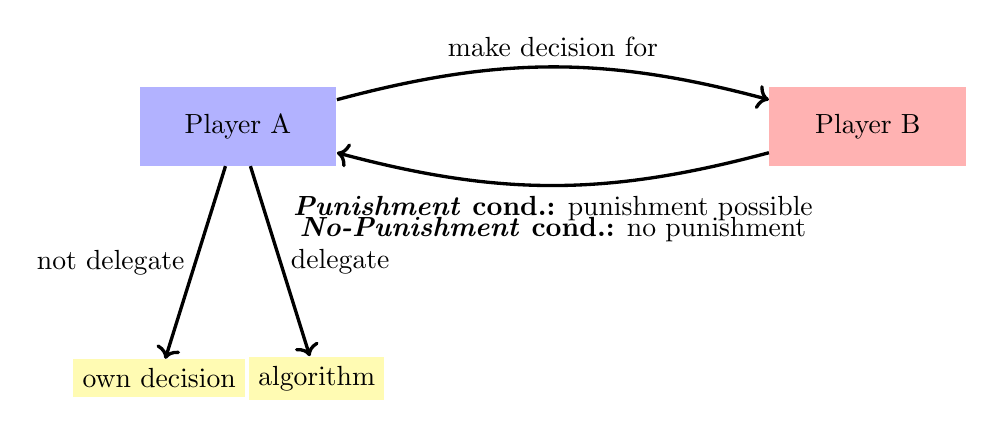
\begin{tikzpicture}[scale=1, every node/.style={scale=1}]
            %boxes
            \node (A) at (1,-3.2) [fill=yellow!30] {algorithm};
            \node (OD) at (-1,-3.2) [fill=yellow!30] {own decision};
            \node (D) at (0,0) [fill=blue!30, minimum width=2.5cm, minimum height=1cm] {Player A};
            \node (E) at (8,0) [fill=red!30, minimum width=2.5cm, minimum height=1cm] {Player B};

            %arrows
            \draw[<-, very thick] (A) to node[right] {delegate} (D);
            \draw[<-, very thick] (OD) to node[left] {not delegate} (D);
            \draw[->, very thick, bend left = 15] (D) to node[above] {make decision for} (E);
            \draw[<-, very thick, bend right = 15] (D) to node[below, align=center] {\textbf{\textit{Punishment} cond.:} punishment possible\\[-1ex]\textbf{\textit{No-Punishment} cond.:} no punishment} (E);

    \end{tikzpicture}
    }
    \label{fig:treatments}
\end{figure}

\subsection*{Sample}

We targeted a balanced design of 80~participants per role per condition, for a planned sample of 320~subjects. The cell size was set to detect, at conventional power, the effects anticipated from the responsibility-avoidance literature; the underlying ex-ante power calculation is reproduced in Appendix~\ref{appendix:pap}. Attrition and subsequent re-matching brought the realised sample to 322 participants ($161$ Player~A and $161$ Player~B), with a CONSORT-style flow diagram broken down by condition and role in Appendix~\ref{appendix:attrition}.
%FB comment: The statement is not backed by evidence. We should say something like: With this sample size, at conventional power, one can detect a treatment effect of X given standard deviation of Y [Perhps do the following calculations and show a figure in the appendix: At 80% power with the given sample size and alpha=0.05, plot the treatment effect size and standard deviation in % of the treatment effect size on the y and x axis or x and y axis]. 
%FB comment: Let's only refer to the CONSORT-style flow diagram at the end of talking about the procedure for player A and player B. Also, let's not call it CONSORT style diagram, let's just stay generic and say that the details of the experimental timeline/procedure can be understood from figure X in the appendix.

The experiment was programmed in oTree~\citep{chen_otree_2016} and run via Prolific. Eligibility followed Prolific's standard quality screens---minimum 95\% prior approval rate, no warnings on file, fluent-English filter, and UK residence---together with a desktop-only restriction (no mobile or tablet) to keep the screen layout consistent across subjects. Player~A spent on average 12~minutes on the study and earned an average bonus of $\pounds 2.49$ on top of the Prolific show-up fee; Player~B spent on average 8~minutes and earned an average bonus of $\pounds 2.30$.\footnote{Bonus computed deterministically from cleaned data per the experimental rules: random-round task payoff (expectation over the uniform draw), belief-about-own-score payoff ($\pounds 0.30$ times the mass placed on the realised score), belief-about-distribution payoff (expectation over the uniform random draw of which score is checked), and---for Player~A in the \textit{Punishment} condition---expected punishment from the matched Player~B's strategy-method choice in the realised cell, with $\pounds 0.10$ per cell of strategy-method punishment cost for Player~B. The bonus excludes the risk-elicitation MPL payoff (raw-data column not retained in the cleaned files); including it would add roughly $\pounds 0.30$--$\pounds 0.50$ per subject.}
%FB comment: The whole "Sample" subsection seems to overlap a lot with the "Sample, Attention and Balance" subsection in the results section. Please avoid repetition and please think about it and recommend where to include this information. It would also be possible to include some info in the design section and some in the results section. Let's discuss a plan first.

\subsection*{Procedure}

\subsubsection*{Player A}

After providing informed consent, Player~A completed ten incentivised rounds of a visual prediction task. In each round, she predicted a person's weight from a facial image and the person's height. Predictions could be entered via slider or typed directly in kilograms, pounds, or stones-and-pounds; no feedback was provided between rounds.\footnote{All individuals depicted in the images had explicitly consented to the use of their photographs for research purposes.} At the end of the experiment, one of the ten rounds was randomly selected for payment: Player~A earned $\pounds 4$ if her prediction in that round was within $10$~lbs of the true weight and $\pounds 2$ otherwise. These initial rounds served three purposes simultaneously: they established a stake from which any later punishment could be deducted; they familiarised Player~A with the task; and they generated the performance data needed to calibrate the algorithm.

The choice of a visual prediction task is deliberate. Algorithm preferences depend sensitively on the algorithm's perceived relative competence~\citep{dietvorst_algorithm_2015,logg_algorithm_2019}; as described below, our design neutralises this concern by calibrating the algorithm to match each subject's individual performance. The visual nature of the task makes algorithmic error plausible and lends credibility to the equal-performance claim, in contrast to purely mathematical tasks where subjects may be sceptical that an algorithm could ever fail~\citep{gogoll_rage_2018}. Predicting body weight from a facial image has been used in earlier experiments~\citep{logg_algorithm_2019} and arguably levels the playing field between human and algorithm: humans have a lifetime of practice at this mapping, while algorithms cannot easily exploit large training corpora here. Finally, we chose a prediction task involving genuine uncertainty rather than a setting with an obvious self-serving motive (as in classic dictator-game variations). This reflects the nature of many real-world applications of algorithms---financial forecasting, medical diagnosis, fraud detection---in which outcomes are inherently uncertain and performance is evaluated ex post.
%FB comment: Add a comment to the provided references here, because I will want to check whether this is precisely what these papers are about. Please do a first check yourself by reading through these papers.

After the ten rounds, Player~A was randomly paired with another participant, Player~B. Player~A was informed that her final, eleventh prediction would not affect her own payoff but would almost entirely determine the payoff of Player~B, who had not completed the prediction task himself: if the prediction fell within 10~lbs of the true weight, Player~B would receive a high payoff ($\pounds 5$); otherwise a low payoff ($\pounds 1$). Player~A then learned that she could either make the prediction herself or delegate it to an algorithm calibrated to mimic her own performance from the first ten rounds, so that on expectation the algorithm would produce the high payoff for Player~B at the same rate as Player~A would.
%FB comment: I would not say that Player A knew that the algorithm would mimic their own success chance. I would say something more neutral, such as "were told that the algithm performed equally well in the first 10 rounds." Also, it is not necessarily true, that even in expectation the algirthm would perform the same as Player A, because Player A could now put more effort. Please rephrase this or leave out this claim.

Concretely, the algorithm draws a Bernoulli outcome with success probability equal to Player~A's empirical accuracy rate over her first ten rounds. A subject who scored 3/10 in the initial rounds thus delegates to an algorithm that produces the high payoff for Player~B with $30\%$ probability. This individual-level Bernoulli calibration is the central design innovation relative to the closest precedent~\citep{feier_hiding_2022}, and it does substantive work in the identification argument. First, it makes the equal-performance claim literally true on average for every subject. Second, it strips any signal value that the delegation decision might otherwise carry about Player~A's beliefs concerning her own ability relative to the algorithm: a Player~B observing the delegation decision has no basis on which to read it as overconfident, lazy, or selfish. This closes off the most plausible third-party signal-extraction channel through which delegation might otherwise insulate the principal from punishment.
%FB comment: It "makes it literally true" for the first 10 rounds, but not necessarily for the last round, right?

The contrast with session-level calibration is consequential. Had the algorithm instead been calibrated to reflect aggregate performance across a pool of participants---as in \citet{feier_hiding_2022}---the delegation choice would be confounded by each subject's beliefs about her own ability relative to the pool. Indeed, \citet{feier_hiding_2022} report that the delegation decision in their setting is largely driven by perceived own performance relative to the algorithm. Pairing the algorithm to each subject individually, and making this common knowledge between Player~A and Player~B, strips this confound out by construction.

In the \textit{Punishment} condition, Player~A was further informed that Player~B could reduce her payoff by up to $\pounds 2$, with the deduction depending on both her delegation decision and the realised outcome. In the \textit{No-Punishment} condition, Player~B had no punishment option. The two delegation options (own decision / algorithm) were presented in random order across subjects, to control for any framing effect of which option appeared first. We attached no monetary cost to delegation: had we done so, no-delegation would have been the rational choice in the \textit{No-Punishment} condition by construction, masking any treatment effect on intrinsic preference. If Player~A chose not to delegate she was asked to make the final prediction and to state her confidence in having earned the high payoff for Player~B; this step was skipped if the algorithm made the prediction.
%FB comment: Here I am worried that the justification for the costlessness of delegation is not strong enough. I would perhaps add that making it costless gets us closer to the intrinstic preference without punishment (but not claim that it is weakly dominant to not delegate...because we do not know which other mechnaisms are at play) and, if true, say that this is standard in the literature.; The last sentence is arbitrary, because the second to last sentence already qualifies the condition under which the confidence was elicited. Let's drop the last sentence.

We then asked Player A to report her beliefs about Player B's punishment in each of the four scenarios resulting from the combination of delegation decision (yes/no) and prediction outcome (high/low payoff for Player B). Beliefs were elicited on the same scale as actual punishment ($\pounds 0$--$\pounds 2$ in $\pounds 0.10$ increments) and the four scenarios were presented in block-wise random order. We chose not to incentivise belief elicitation for three reasons. First, only two of the four scenarios remain payoff-relevant after the delegation decision, making the others purely hypothetical. Second, an incentivised mechanism could induce hedging behaviour. Third, an incentive-compatible scoring rule across four scenarios would have substantially increased task complexity. Because we are nonetheless interested in comparing punishment beliefs to actual punishment, we included an attention check on the belief-elicitation screen.\footnote{Subjects who failed the attention check are excluded from belief-related analyses, as preregistered.} In the \textit{No-Punishment} condition, no punishment was possible; we elicited beliefs about hypothetical punishment to maintain consistency across treatments.
%FB comment: Here I want to make a general comment: We have to think about how we talk about the pre-registration. Ideally, I would like to link it once in the beginning and then not refer to it, unless I deviate from the preregistration. I have put the pre-registration into a folder "pre-registration". Please read it and suggest all edits you would make to the draft based on it. The analysis should not change, we should only disclose if we deviate strongly from the pre-registration.

Player~A was then asked to assess her own performance in the first ten rounds by assigning a probability mass (summing to $100\%$) to each possible score from $0$ to $10$. This elicitation was incentivised: Player~A earned an additional $\pounds 0.30$ with the probability she had assigned to her actual score.\footnote{This mechanism is not incentive-compatible for risk-neutral participants. In practice only one subject assigned the full probability mass to a single score, suggesting that hedging considerations were modest.} She was also asked to estimate the population distribution of scores by assigning a share to each possible score from $0$ to $10$; one score was randomly drawn at the end of the experiment and Player~A earned $\pounds 0.30$ if her estimate for that score was within five percentage points of the realised population share.
%FB comment: The assessment of own performance will be influenced by already having received the information that the algorithm has performed the same. We should have probably elicited these performance related beliefs prior to the delegation decision, etc. Can you think of any reasons why it may still be a good idea to have done it afterwards, e.g. the delegation deciison is done, knowing that performance in the first 10 rounds was the same, so we are interested in the performance belief after having received that information. Perhaps to justify the elicitation of beliefs about others' performance, what could be a reason? To assess overconfidence/confidence relaive to others, but why? Regarding the footnote, I would not say that hedging motives were modest, because most people hedged in a sense by apportioning postivie probability mass for multiple options.

Finally, we elicited risk preferences using an incentivised multiple price list in the style of \citet{holt_risk_2002} and administered a short questionnaire on socio-demographic characteristics and technology affinity, before presenting Player~A with her preliminary payoff. Figure~\ref{fig:design_playerA} summarises the experimental timeline for Player~A.

\subsubsection*{Player B}

After providing informed consent, Player~B was told that he had been randomly matched with a Player~A and was introduced to the task Player~A had completed. He learned that his own payoff would be determined by the outcome of Player~A's eleventh prediction---$\pounds 5$ if it fell within 10~lbs of the true weight and $\pounds 1$ otherwise---while Player~A's payoff depended solely on her performance in the initial ten rounds. Crucially, Player~B was also told that Player~A could delegate the eleventh prediction to an algorithm calibrated to perform equally well as Player~A in the earlier rounds, and that Player~A herself was aware of this equal-performance calibration. The equal-performance claim is therefore common knowledge between the two players, a feature on which our identification argument rests.
%FB comment: I don't like "eleventh" prediction. Maybe "final", "additional", etc? 

In the \textit{Punishment} condition, Player~B could choose to reduce Player~A's payoff by up to $\pounds 2$ in $\pounds 0.10$ increments, at a personal cost of $\pounds 0.10$ per scenario in which positive punishment was chosen.\footnote{The cost is fixed per scenario rather than proportional to the punishment level, so that strictly positive punishment is always costly relative to no punishment but the cost does not increase with the severity of the sanction.} We elicited punishment decisions for all four combinations of delegation (yes/no) and outcome (high/low payoff for Player~B) via the strategy method, implementing only the decision matching the realised combination. The strategy method is essential to our power: a between-subject elicitation across cells would have required roughly four times the sample to detect cell-level differences at comparable power, well beyond our recruitment budget.\footnote{The strategy method may yield different absolute punishment levels than direct elicitation; we discuss the implications and a possible direct-method companion as future work in Section~\ref{conclusion}.} Because the punishment decision is the central outcome variable, we included an attention check on the punishment-elicitation screen.\footnote{The check asked the subject to confirm a numerical aspect of the payoff structure that had been displayed on the previous screen. Subjects failing this check are excluded from punishment-related analyses, as preregistered.} In the \textit{No-Punishment} condition, where actual punishment was not possible, we elicited hypothetical punishment decisions on the same scale to keep the experimental flow comparable across conditions. Player~B's perceptions of task difficulty, his risk preferences, and a short questionnaire followed, before he was presented with his final payoff. Figure~\ref{fig:design_playerB} summarises the experimental timeline for Player~B.
%FB comment: Can we say that the cost lied in foregoing an addition 0.10 pounds. I do not want the reader to think that the punishment was deducted. Also, please do not claim the we had a tight research budget or that the sample size would need to be four times higher. It's fine to keep a sentence that the strategy method gives us more power, but don't elaborate so much.

Once Player~B's decisions had been recorded, Player~A's final payoff was calculated and all participants were paid on the day of participation.

\subsection*{Hypotheses}

Our design tests two preregistered hypotheses, both grounded in the literature on responsibility avoidance through delegation~\citep{bartling_shifting_2012,coffman_intermediation_2011,oexl_shifting_2013,hamman_self-interest_2010,hill_does_2015,steffel_passing_2016} and on responsibility attributions to algorithmic decision-makers~\citep{feier_hiding_2022,kirchkamp_sharing_2019,gogoll_rage_2018}.

\begin{description}
\item[H1 (Delegation):] The introduction of potential punishment increases the likelihood that Player~A delegates the decision to the algorithm.
\item[H2 (Punishment):] Conditional on a low-payoff outcome for Player~B, Player~A is punished less when she delegated the decision to the algorithm than when she made it herself.
\end{description}

H1 is grounded in robust empirical evidence that responsibility avoidance shapes delegation decisions involving human intermediaries. \citet{bartling_shifting_2012} also show that subjects are more likely to delegate morally consequential decisions even to a die roll---an early form of delegation to a non-intentional agent---suggesting that responsibility avoidance persists when the agent lacks intentionality. \citet{feier_hiding_2022} find no significant difference in the propensity to delegate to a human versus an algorithmic agent, suggesting that the nature of the agent may matter less than the opportunity to shift responsibility.
%FB comment: maybe leave out "robust"? If we made the literature appear to be too conclusive, what would be our contribution?; For the Feier et al paper, what is lacking a bit here is the relationship to H1. The propensity to delegate decisions to AI or human is the same, but is it higher under punishment than without punishment for both or not?

H2 mirrors H1 on the punishment side. \citet{bartling_shifting_2012} find that delegation to a randomisation device still allows decision-makers to avoid some punishment, although less so than delegation to another human. \citet{feier_hiding_2022} find that decision-makers are rewarded less when a negative outcome is directly attributable to their own action, compared to when it results from an algorithm to which they delegated. Their study differs from ours in three respects, however: a different task; an emphasis on reward differentials rather than punishment; and---most consequentially---a design that does not control for relative performance at the individual level. As a result, in their setting the delegation decision carries a strong signal about Player~A's beliefs concerning her own ability relative to the algorithm; a failure to delegate may then be punished as overconfidence rather than as direct responsibility-taking, contaminating the inference about responsibility-shifting per se.
%FB: comment: This is a general comment: Do we have to talk about why we chose only punishment to be possible, but no reward? In what way does it matter? In what way could it be better to use punishment? Do we talk about it earlier that blame/responsibility is usually operationalized/measure through punishment? If so, should we repeat this at some point or not?

\subsection*{Identification}
%FB comment: I am wondering whether this subsection should be integrated together with the Hypothesis subsection? Would that be possible or are there strong reasons against it?

The design pins down two distinct quantities. The within-subject comparison across the four (delegation, outcome) cells of Player~B's strategy-method punishment isolates the conditional-on-outcome effect of delegation on punishment, holding fixed the realised consequences for Player~B (the test of H2). The between-subject comparison of Player~A's delegation rate across \textit{Punishment} and \textit{No-Punishment} isolates the effect of the punishment possibility on the propensity to delegate, holding fixed every other feature of the decision environment (the test of H1). The first comparison absorbs all between-subject heterogeneity in Player~B's punishment proclivity; the second exploits the punishment manipulation as the only between-subject difference.

Two further design features deserve note. First, although the prediction task affects Player~B's payoff, the incentives of the two players are nominally aligned: Player~A has no direct financial interest in Player~B receiving the low payoff, and a successful prediction strictly weakens her own expected punishment.\footnote{In the \textit{Punishment} condition, a better outcome for Player~B reduces expected punishment for Player~A; in the \textit{No-Punishment} condition there is no punishment to reduce. Either way, Player~A's incentives are weakly aligned with Player~B's.} A standard intention-based punishment motive should therefore have less bite here than in dictator-game settings where the decision-maker can choose to be selfish. Second, although the underlying decision (a prediction under uncertainty) is not itself moral, the setup nonetheless qualifies as part of the \textit{moral domain} as defined in the algorithm-aversion literature~\citep{gogoll_rage_2018}: Player~A's choice imposes monetary externalities on a third party, and a poor decision causes real, albeit modest, monetary harm. The implications of these two design choices for the interpretation of our results are taken up in Section~\ref{results}.
%FB comment: Can we justify why t makes sense to have the incentives aligned here? Many AI applications are of this aligned nature, no?

\section{Results} \label{results}

Data collection took place between February and June 2023 through the British online platform Prolific, with all participants recruited from the United Kingdom.\footnote{EXCLUSION CRITERIA: leave a comment for Felix to insert later} A total of $322$ subjects were recruited ($161$ assigned to Player~A, $161$ to Player~B).\footnote{We preregistered the collection of data from $320$ participants ($80$ subjects per role per treatment). Due to attrition and subsequent re-matching we recruited an extra pair in the \textit{Punishment} condition.} On average, Player~A spent $12$ minutes completing the experiment and earned an average bonus of $\pounds 2.49$ on top of the Prolific show-up fee, while Player~B spent approximately $8$ minutes and earned an average bonus of $\pounds 2.30$. Treatment randomization was effective, as demonstrated by the balance across observable characteristics (Appendix~\ref{appendix:sum_stats}, Table~\ref{tab:treatment_balance}). A flow diagram showing recruitment, attrition, attention-check exclusion, and the analysis sample, broken down by condition and role, appears in Appendix~\ref{appendix:attrition}; in particular, attrition rates do not differ meaningfully across the \textit{Punishment} and \textit{No-Punishment} conditions.

We preregistered exclusion of subjects who failed the attention check on the screen at which their main outcome variable was elicited. For Player~A, this is the belief-elicitation screen; for Player~B, the punishment-elicitation screen. Of $161$ Player~Bs, $135$ pass the attention check ($83.9\%$); the corresponding pass rate for Player~A is $131/161$ ($81.4\%$). All main results are robust to including subjects who fail the attention check; we report these robustness checks in Appendix~\ref{appendix:regs}.
\todo[inline]{FB: maybe move to first set of results. Also the appendix does not show anything and the default should be including everyone.}

\subsection*{Result~1: Punishment reduces delegation} \label{sec:result1}

\paragraph{Headline.} In the \textit{Punishment} condition, where Player~B can punish, $42.5\%$ of Player~As delegated the decision to the algorithm. In the \textit{No-Punishment} condition, where punishment is impossible, $59.3\%$ delegated. Figure~\ref{fig:delegation_shares} illustrates the difference. The introduction of potential punishment thus significantly \textit{reduces} the likelihood of delegation to the algorithm (Pearson Chi-squared, $p=0.033$; Fisher's exact, $p=0.041$).\footnote{The preregistration is non-directional on H1; the realized direction is opposite to that anticipated by the responsibility-avoidance literature on which the hypothesis was grounded. We report two-sided tests throughout the body of the paper. The full set of preregistered tests, the deviations from each, and the rationale appears in Appendix~\ref{appendix:preregistration}.}\footnote{A within-subject corroborator points the same direction. Player~As in the \textit{No-Punishment} condition were asked, after their actual delegation decision, the hypothetical question of whether they would have delegated had punishment been possible. Among the $81$ respondents, $12$ would have stopped delegating under hypothetical punishment while only $5$ would have started, yielding a hypothetical delegation rate of $50.6\%$ (within-subject McNemar's test $p=0.090$). Hypothetical responses elicited after the actual decision are subject to motivated reasoning; the within-subject pattern complements rather than substitutes for the between-subject test.}

\medskip
\noindent\textbf{Result~1.} \textit{The possibility of punishment significantly reduces the likelihood that Player~A delegates the decision to the algorithm.}
\medskip

\begin{figure}[!htbp]
    \centering
    \caption{Delegation shares by condition}
    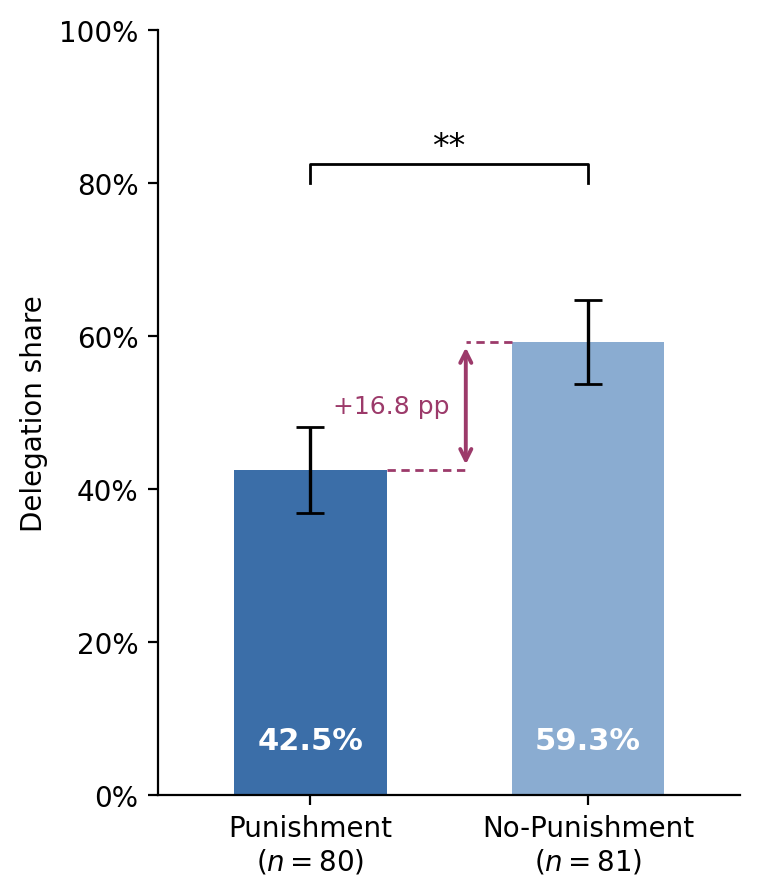
\includegraphics[width=0.5\linewidth]{figures/delegation_shares.png}
    \label{fig:delegation_shares}
    \begin{minipage}{0.6\linewidth}
    \footnotesize
    \textit{Note:} Bars show the share of Player~As who delegated the final prediction to the algorithm in each between-subject condition. The two-sided difference is significant at the $5\%$ level under both a Pearson Chi-squared test ($p=0.033$) and a Fisher's exact test ($p=0.041$). The preregistration does not specify a test direction; the realized effect reverses the sign anticipated by the responsibility-avoidance literature on which the hypothesis was grounded.
    \end{minipage}
\end{figure}

This result not only fails to support \textit{Hypothesis~1}; it points in the opposite direction. The responsibility-avoidance literature, on which H1 rests, would predict the introduction of punishment to make delegation \textit{more} attractive as a tool for shifting responsibility. We instead observe a sizeable reduction in delegation when punishment is on the table. Before turning to candidate mechanisms for this reversal in Section~\ref{sec:mechanism}, we first establish that the effect is robust and document its empirical structure.

\paragraph{With controls.} Table~\ref{tab:del_decision_determinants} reports estimates from a Logit model of the delegation decision. Column~(1) reports the unconditional treatment effect; Column~(2) adds Player~A's task performance and a vector of socio-demographic and technology-affinity controls. The treatment effect is robust: the coefficient on the \textit{No-Punishment} indicator is $0.68$ ($p=0.034$, two-sided) in the unconditional specification and $0.76$ ($p=0.023$, two-sided) with controls. The full set of estimated coefficients is reported in Appendix Table~\ref{tab:reg_delegation}.

\begin{table}[!htbp]
\centering
\scriptsize
\caption{Determinants of the delegation decision}
\label{tab:del_decision_determinants}
\begin{tabular}{@{\extracolsep{5pt}}lcccc|c}
\\[-1.8ex]\hline
\hline \\[-1.8ex]
& \multicolumn{5}{c}{Dependent variable: \textit{Delegation}}\\[0.1cm]
& \multicolumn{4}{c}{\textit{Full sample}} & \textit{Passers} \\
\\[-1.8ex] & (1) & (2) & (3) & (4) & (5) \\
\hline \\[-1.8ex]
 Punishment indicator & $-0.423^{**}$ & $-0.435^{**}$ & $-0.472^{**}$ & $-0.448^{**}$ & $-0.517^{**}$ \\
  & $(0.199)$ & $(0.204)$ & $(0.206)$ & $(0.205)$ & $(0.230)$ \\[0.1cm]
 Task performance &  &  & $-0.119$ &  & $-0.158^{*}$ \\
  &  &  & $(0.079)$ &  & $(0.086)$ \\[0.1cm]
 Perceived performance &  &  &  & $-0.072$ &  \\
  &  &  &  & $(0.056)$ &  \\[0.1cm]
 Age &  & $-0.002$ & $-0.002$ & $-0.002$ & $0.002$ \\
  &  & $(0.009)$ & $(0.009)$ & $(0.009)$ & $(0.010)$ \\[0.1cm]
 Female &  & $0.175$ & $0.222$ & $0.212$ & $0.407$ \\
  &  & $(0.227)$ & $(0.228)$ & $(0.229)$ & $(0.254)$ \\[0.1cm]
 Socio-economic status &  & $-0.038$ & $-0.035$ & $-0.031$ & $-0.082$ \\
  &  & $(0.071)$ & $(0.072)$ & $(0.071)$ & $(0.079)$ \\[0.1cm]
 Went to uni &  & $0.036$ & $0.059$ & $0.025$ & $0.124$ \\
  &  & $(0.227)$ & $(0.225)$ & $(0.227)$ & $(0.247)$ \\[0.1cm]
 Technology score &  & $-0.069$ & $-0.048$ & $-0.062$ & $0.014$ \\
  &  & $(0.092)$ & $(0.095)$ & $(0.092)$ & $(0.107)$ \\[0.1cm]
 Leadership position &  & $0.404^{*}$ & $0.422^{*}$ & $0.399^{*}$ & $0.253$ \\
  &  & $(0.225)$ & $(0.226)$ & $(0.225)$ & $(0.253)$ \\[0.1cm]
 Constant & $0.234^{*}$ & $0.452$ & $0.714$ & $0.716$ & $0.651$ \\
  & $(0.141)$ & $(0.545)$ & $(0.584)$ & $(0.593)$ & $(0.656)$ \\[0.1cm]
\hline \\[-1.8ex]
 AME of Punishment (pp) & $-16.8^{**}$ & $-16.8^{**}$ & $-18.0^{**}$ & $-17.2^{**}$ & $-19.4^{**}$ \\
  & $(p=0.031)$ & $(p=0.030)$ & $(p=0.019)$ & $(p=0.026)$ & $(p=0.021)$ \\
 N & $161$ & $159$ & $159$ & $159$ & $130$ \\
 Pseudo $R^2$ & $0.020$ & $0.039$ & $0.049$ & $0.047$ & $0.064$ \\
\hline
\hline \\[-1.8ex]
\multicolumn{6}{c}{\begin{minipage}{0.85\textwidth}\footnotesize \textit{Note:} Coefficients from a Probit regression of the delegation decision on the Punishment indicator and a set of controls. Robust (HC1) standard errors in parentheses. Significance: $^{*}\,p<0.10$; $^{**}\,p<0.05$; $^{***}\,p<0.01$ (two-sided). Due to missing socio-demographic data, two subjects are dropped in Columns~(2)--(5). The \textit{AME of Punishment} reports the average change in the predicted probability of delegation from introducing the punishment possibility, in percentage points.\end{minipage}}
\end{tabular}
\end{table}


\paragraph{Robustness.} The treatment effect survives several further checks. First, controlling for Player~A's overconfidence (defined as the weighted-average belief about own performance minus actual performance) leaves the \textit{No-Punishment} coefficient essentially unchanged ($0.77$, $p=0.022$); overconfidence itself is not significantly associated with delegation ($p=0.272$). Second, order effects are localised to the \textit{Punishment} condition: presenting the algorithm option first roughly doubles delegation ($52.5\%$ vs $32.5\%$ when the own-decision option is first; $\chi^2$ $p=0.070$), while the \textit{No-Punishment} condition shows no order effect ($p=0.674$); the treatment $\times$ order interaction is not significant ($p=0.115$), so the H1 finding is not driven by interaction with order. Third, relaxing the preregistered attention-check exclusion does not change the result. The full robustness specification is reported in Appendix Table~\ref{tab:reg_delegation_robustness}.

\paragraph{Heterogeneity by performance.} Within the \textit{Punishment} condition, Player~As who performed better on the first ten rounds were less likely to delegate. The Pearson correlation between the score in the first ten rounds and the probability of delegation is $-0.19$ (two-sided $p=0.092$); the corresponding regression coefficient in Column~(3) of Table~\ref{tab:del_decision_determinants} is $-0.61$ (two-sided $p=0.010$). The strengthening of the relationship in the regression reflects, in part, the attention-check restriction (Column~(3) is identified off $n=60$ Punishment-attention-pass subjects, while the raw correlation uses all $80$ Punishment subjects). In the \textit{No-Punishment} condition, no comparable relationship between performance and delegation is observed. Figure~\ref{fig:performance_delegation_scatter} visualises this asymmetry. We flag this paragraph as the empirical hint that motivates the process-ownership mechanism developed in Section~\ref{sec:mechanism}: the condition effect is concentrated among Player~As who, conditional on punishment being on the table, prefer to take a personal stake in producing a good outcome for Player~B.

\begin{figure}[!htbp]
    \centering
    \caption{Delegation share by performance and condition}
    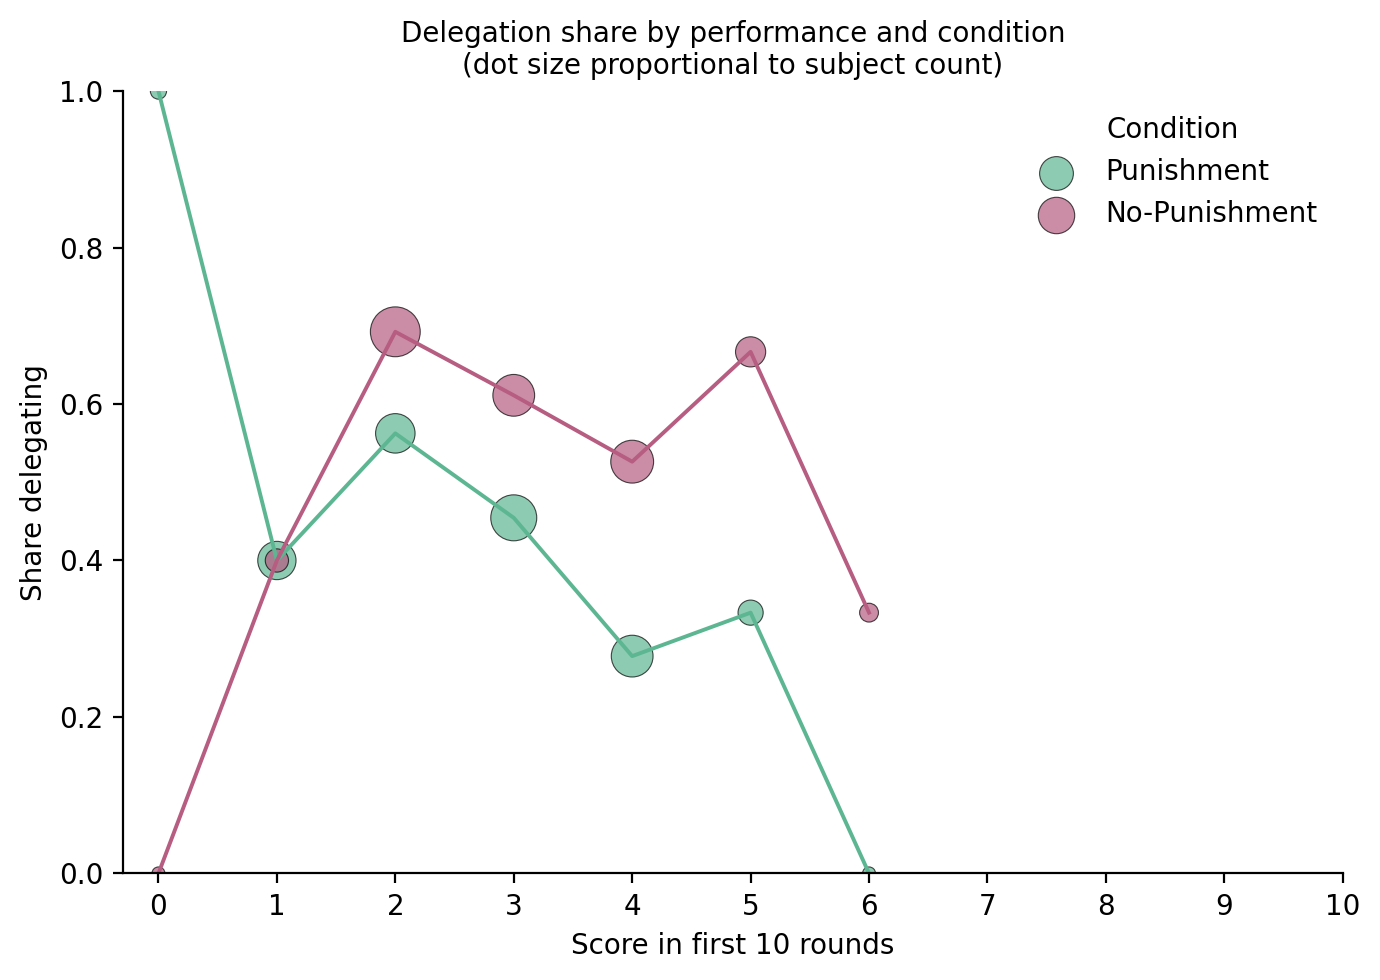
\includegraphics[width=0.7\linewidth]{figures/performance_delegation_scatter.png}
    \label{fig:performance_delegation_scatter}
    \begin{minipage}{0.85\linewidth}
    \footnotesize
    \textit{Note:} Each point reports the share of Player~As at the corresponding first-ten-rounds score who delegated the final prediction. Dot size is proportional to the number of subjects at that score. The downward slope in the \textit{Punishment} condition is the Pearson $r=-0.19$ ($p=0.092$); no comparable slope in \textit{No-Punishment}. Restricted to attention-check passers.
    \end{minipage}
\end{figure}

\subsection*{Result~2: We cannot reject equal punishment of delegated and self-made decisions} \label{sec:result2}

\paragraph{Headline.} We now turn to Player~B's punishment behavior in the \textit{Punishment} condition. Punishment in all four (delegation, outcome) cells of the strategy method is significantly greater than zero, and Player~Bs punish more for low-payoff outcomes than for high-payoff outcomes---an indication that punishment carries informational content rather than being noise; $41.8\%$ of Player~Bs nonetheless do not punish in any of the four scenarios. Conditional on the outcome, however, Player~A is not significantly differently punished depending on the delegation decision. When Player~B receives the high payoff, average punishment is $\pounds 0.311$ for delegated decisions and $\pounds 0.310$ for self-made decisions---a difference of one-tenth of a penny. When Player~B receives the low payoff, average punishment is $\pounds 0.494$ when Player~A delegated versus $\pounds 0.571$ when she made the decision herself; this difference points in the H2 direction but is far from significant (paired $t$-test $p=0.153$; Wilcoxon signed-rank $p=0.533$). The same picture obtains when measuring punishment frequencies rather than amounts: Player~Bs neither punish delegated decisions more harshly, nor do they punish them more frequently (Appendix Figure~\ref{fig:punishment_frequencies}). As preregistered, the within-subject test is identified off the $67$ Player~Bs in the \textit{Punishment} condition who passed the attention check; the result is essentially identical when these subjects are included (mean difference $\pounds 0.071$ vs $\pounds 0.077$; paired $t$-test $p=0.131$ vs $p=0.153$; Appendix Table~\ref{tab:reg_punishment_robustness}).

\medskip
\noindent\textbf{Result~2.} \textit{Conditional on the outcome for Player~B, we cannot reject the hypothesis that Player~A is punished equally for delegated and self-made decisions. A TOST equivalence test rules out moderate insulation effects (those exceeding $\pounds 0.20$, or $10\%$ of the maximum punishment) at $\alpha = 0.05$, but we cannot rule out smaller insulation effects.}
\medskip

\begin{figure}[!htbp]
    \centering
    \caption{Punishment by Player~B and beliefs about punishment by Player~A}
    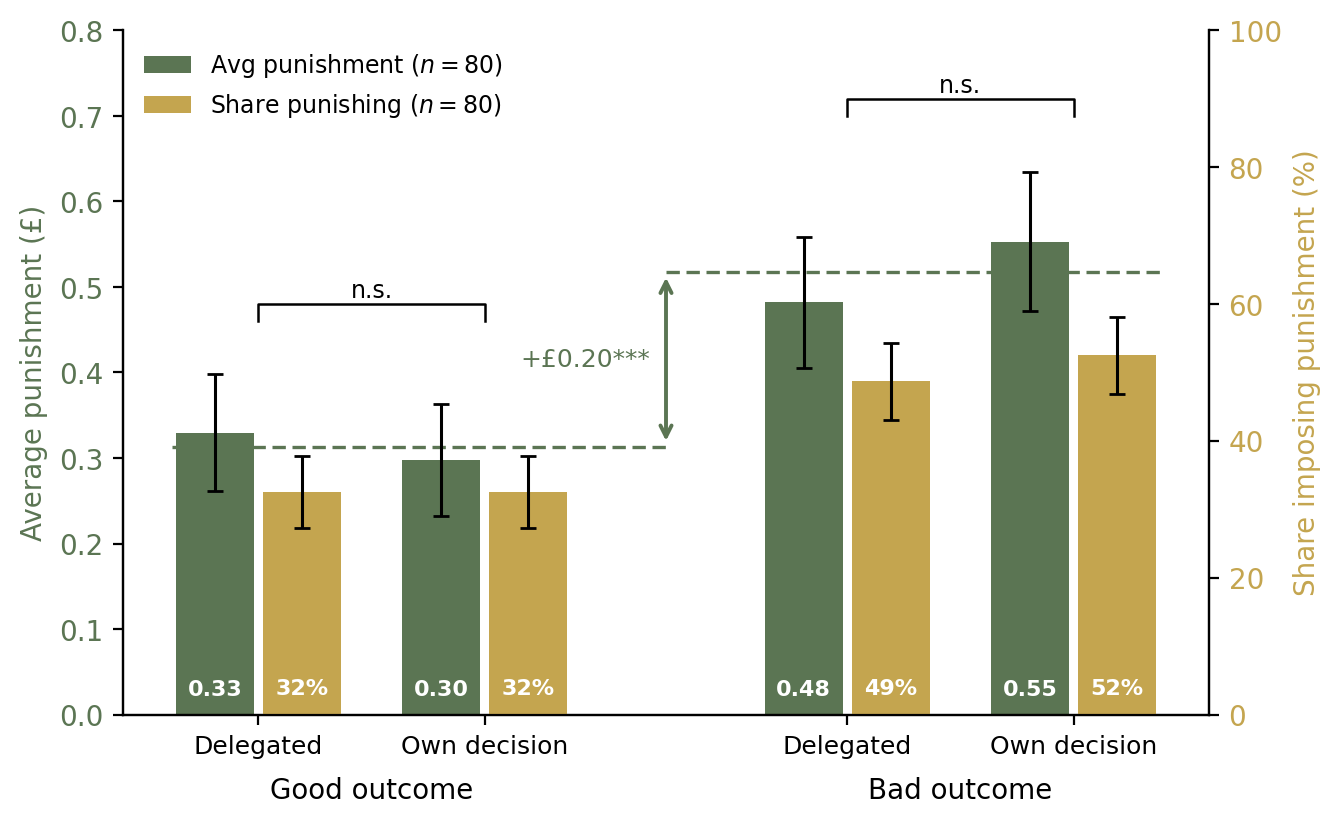
\includegraphics[width=0.6\linewidth]{figures/punishment.png}
    \label{fig:punishment}
    \begin{minipage}{0.85\linewidth}
    \footnotesize
    \textit{Note:} Average punishment chosen by Player~B (solid bars) and average belief about punishment held by Player~A (hollow bars) for each of the four scenarios. Bars are reported in pounds and standard errors are reported as error bars. Beliefs are elicited prior to learning the realized outcome and on the same scale as the punishment decision; the belief overlay is analysed in Section~\ref{sec:mechanism}.
    \end{minipage}
\end{figure}

\paragraph{Equivalence (TOST).} We can refine the negative result with a positive equivalence claim. A two one-sided test (TOST) at the $\pm \pounds 0.20$ bound---against the null that the true insulation effect exceeds $10\%$ of the maximum punishment---rejects in both the bad-outcome cell ($p = 0.012$) and the good-outcome cell ($p < 0.001$). At a tighter $\pm \pounds 0.10$ bound, equivalence cannot be established ($p = 0.332$ for the bad-outcome cell). In our setting we can therefore rule out moderate insulation effects (above $\pounds 0.20$ per cell) with high confidence, but cannot rule out small ones below this bound.

\paragraph{What predicts punishment?} Appendix Table~\ref{tab:reg_punishment} reports a regression of chosen punishment on a delegation indicator, an outcome indicator, their interaction, Player~B's beliefs about Player~A's performance, and a vector of socio-demographic controls. The interaction term is small and statistically insignificant ($p=0.137$), confirming the bivariate result. Punishment is also independent of Player~B's belief about Player~A's performance: across all four cells, Pearson correlations between cell-specific chosen punishment and Player~B's weighted-average belief about Player~A's score are essentially zero ($|r| \le 0.03$, all $p > 0.8$). This rules out the alternative explanation that Player~Bs who think Player~A is more capable systematically punish less (or more); punishment is not driven by performance-conditional inference about Player~A.\footnote{Post-experiment Likert measures provide a tentative attitudes--behavior link. Among the $44$ Player~Bs who passed the attention check and completed the post-experiment questions, those who reported that Player~A should feel more responsible for the decision punish self-made good outcomes more relative to delegated good outcomes (Pearson $r=0.36$, $p=0.015$ between the responsibility Likert and the within-subject difference $\textit{punish\_nodel\_good} - \textit{punish\_del\_good}$); the corresponding pattern in the bad-outcome cell goes in the same direction but is not significant ($r=0.24$, $p=0.114$). When asked directly who should be accountable for AI-generated decisions, $66\%$ of these subjects identified deploying companies as primarily accountable, $18\%$ developers, $14\%$ end-users, and only one named government or regulatory bodies. The sub-sample is small ($n=44$); we treat these patterns as suggestive.}

\paragraph{Interpretation.} The fact that we cannot reject equal punishment for delegated and self-made decisions is consistent with our specific design: because the algorithm is calibrated at the individual level and this calibration is common knowledge, the delegation decision in our setting carries no signal about Player~A's belief in her own ability relative to the algorithm. A natural intention-based punishment motive is therefore muted: Player~B has no obvious basis on which to read the delegation decision as overconfident, lazy, or selfish. By the same token, however, this design choice limits the test of H2 to a setting in which the most studied path through which delegation might insulate from punishment---signal extraction by the third party---is closed off by construction. The complementary reading is that responsibility shifting through delegation may operate more strongly when relative performance is uncertain (as in \citealt{feier_hiding_2022}); we discuss in Section~\ref{conclusion} why a follow-up study that varies relative-performance calibration directly is the natural way to map this margin.

\subsection*{Mechanism: candidate explanations for the H1 reversal} \label{sec:mechanism}

The direction of Result~1 reverses the standard prediction of the responsibility-avoidance literature, in which the prospect of punishment should make delegation \textit{more} attractive, not less. Because the reversal was not preregistered, the analyses in this subsection are exploratory and we treat the supported mechanisms as candidate hypotheses rather than as established. We consider four candidates---anticipated differential punishment (M1), effort to outperform the algorithm (M2), process ownership (M3), and experimenter demand (M4)---and weigh each against the data, taking care to distinguish what we can rule out from what we can only flag as consistent. Before turning to the four candidates, we lay out the belief evidence on which several of them rely, separating beliefs about Player~A's task performance from beliefs about Player~B's punishment.

\paragraph{Performance beliefs.} Both players overestimate Player~A's task performance. The true mean overall score in the first ten rounds is $2.93/10$, while Player~A's weighted-average belief about her own score is $4.76$ (overestimate of $1.84$ score points) and Player~B's weighted-average belief about Player~A's score is $4.32$ (overestimate of $1.40$ score points). The overestimation is therefore not a Player-A-specific or Player-B-specific artefact, but a feature of the elicitation. Performance beliefs do not enter the M1 ruling-out argument below; we report them here as a sanity check on the elicitation rather than as evidence on the mechanism.

\paragraph{Punishment beliefs.} \label{sec:beliefs} After making the delegation decision but before learning the outcome, we elicited Player~A's beliefs about Player~B's punishment in each of the four scenarios. Two patterns emerge. First, Player~As substantially \textit{overestimate} the level of punishment they will face: average expected punishment exceeds average realized punishment in every scenario (Figure~\ref{fig:punishment}, hollow bars). Second, however, Player~As correctly anticipate the \textit{relative} pattern of punishment: they expect no significant difference in punishment between delegated and non-delegated decisions, conditional on outcome---a pattern that closely tracks the actual punishment behavior of Player~B documented in Result~2. \textit{It is this relative-pattern finding---on punishment beliefs alone---that rules out a simple anticipation mechanism for Result~1.} If Player~A had reduced delegation in the \textit{Punishment} because she anticipated being punished more harshly for delegation than for self-made decisions, we would expect to see this asymmetry in the elicited beliefs. We do not.

\paragraph{Within-subject consistency and asymmetric belief patterns.} Despite the weakness of the elicitation, punishment beliefs carry within-subject information. Column~(3) of Table~\ref{tab:del_decision_determinants} reports a Logit regression of delegation on Player~A's belief difference (\textit{no delegation} minus \textit{delegation}) for each outcome, restricted to the \textit{Punishment} condition. Coefficients on both belief differences are positive: a Player~A who expects to be punished more for non-delegation than for delegation in a given outcome is more likely to delegate. The coefficient on the good-outcome belief difference is significant at conventional levels ($1.58$, two-sided $p=0.033$); the coefficient on the bad-outcome belief difference is positive but noisier ($0.94$, two-sided $p=0.21$). The within-subject signal is asymmetric across cells (Figure~\ref{fig:belief_distributions}): the single significant difference between delegators and non-delegators is in the \textit{self decision + good outcome} cell, where delegators expect punishment of $\pounds 0.82$ while non-delegators expect only $\pounds 0.32$ ($t$-test $p=0.006$, Mann-Whitney $p=0.019$); for the other three cells the gap is small and not significant. Because beliefs were elicited after the delegation decision and the elicitation was unincentivised, we cannot rule out that subjects rationalised their choice by holding consistent post-hoc beliefs; the within-subject correlation is consistent with the standard interpretation that anticipated punishment shapes delegation, but does not identify the causal direction.

\begin{figure}[!htbp]
    \centering
    \caption{Player A beliefs about Player B punishment, by delegation choice}
    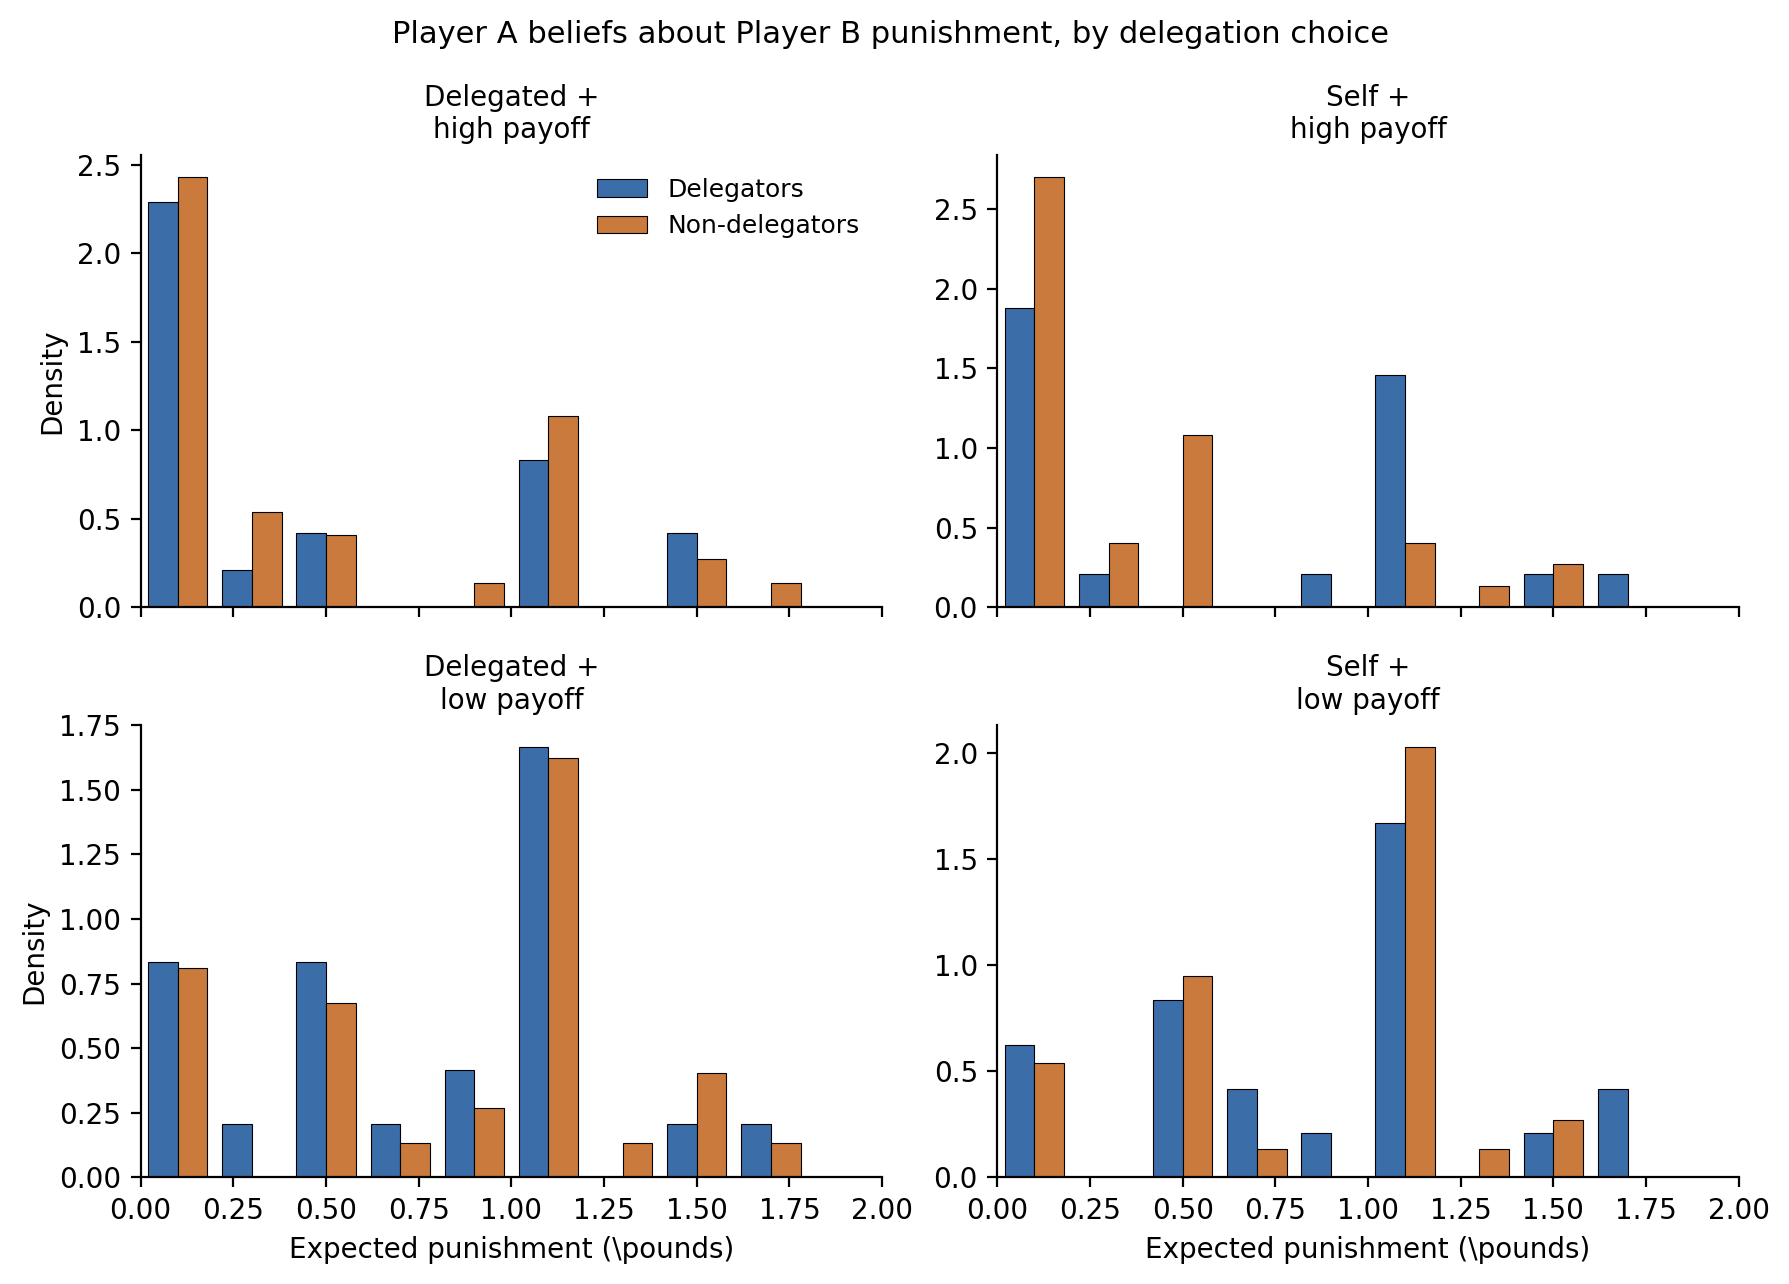
\includegraphics[width=0.85\linewidth]{figures/belief_distributions.png}
    \label{fig:belief_distributions}
    \begin{minipage}{0.9\linewidth}
    \footnotesize
    \textit{Note:} Distribution of Player~A's expected punishment from Player~B in each of the four (delegation, outcome) cells, separately for Player~As who actually delegated (blue) and those who did not (orange). \textit{Punishment} condition, attention-check passers ($n_{\text{deleg}}=24$, $n_{\text{nodeleg}}=37$). The only cell with a statistically significant difference is \textit{self decision + good outcome} (top right): delegators expected $\pounds 0.82$ vs non-delegators $\pounds 0.32$ ($t$-test $p=0.006$).
    \end{minipage}
\end{figure}

\paragraph{(M1) Anticipated punishment for delegation.} A Player~A who expects to be punished more harshly for a delegated decision than for a self-made decision will rationally delegate less when punishment is on the table. The punishment-belief evidence above shows that Player~As do not on average anticipate harsher punishment for delegated decisions, and Player~B does not in fact deliver such punishment (Result~2). M1 is therefore inconsistent with both the elicited beliefs and the realized punishment, and we view this candidate as ruled out by the available evidence.

\paragraph{(M2) Effort exertion to outperform the algorithm.} An alternative mechanism is that the prospect of punishment motivates Player~A to exert greater effort on the final prediction, in the hope of personally producing the high payoff. Although our design controls for relative performance based on the first ten rounds---making the algorithm and Player~A equivalent in expectation on the final prediction---potential punishment could in principle shift Player~A's effort margin. The data are inconsistent with the simple form of this story. Among Player~As who chose not to delegate, those in the \textit{No-Punishment} condition (where punishment is not possible) outperformed those in the \textit{Punishment} condition: $45.5\%$ of non-delegating Player~As in the \textit{No-Punishment} condition earned the high payoff for Player~B, compared to $21.7\%$ in the \textit{Punishment} condition. This difference is not driven by ex-ante performance differences across the first ten rounds (\textit{No-Punishment}: $3.12/10$; \textit{Punishment}: $2.98/10$; two-sided $p=0.66$); the cross-condition mean score in the first ten rounds is $2.93/10$ overall and statistically indistinguishable across conditions (Figure~\ref{fig:performance}), so the M2-relevant gap among non-delegators reflects selection on delegation rather than ex-ante condition differences.\footnote{Measuring performance change as the difference between the average absolute prediction error across the first ten rounds and the absolute prediction error on the final prediction, we find that Player~As in the \textit{No-Punishment} condition improve their performance from rounds~1--10 to round~11, whereas Player~As in the \textit{Punishment} condition do not improve. Because all Player~As across both conditions faced the same image on the final prediction, this differential improvement cannot be attributed to task-specific variation. We caveat that the comparison is between selected non-delegator subsamples, not between random subsets of all Player~As; selection on the very outcome we are measuring is a known limit of this comparison.} Counter-intuitively, increased effort thus appears concentrated among non-delegators in the \textit{No-Punishment} condition, where punishment is \textit{not} on the table---incompatible with a story in which Player~A in the \textit{Punishment} condition tries especially hard to outperform the algorithm in order to avoid punishment.

\begin{figure}[!htbp]
    \centering
    \caption{Performance in the first ten rounds, by treatment}
    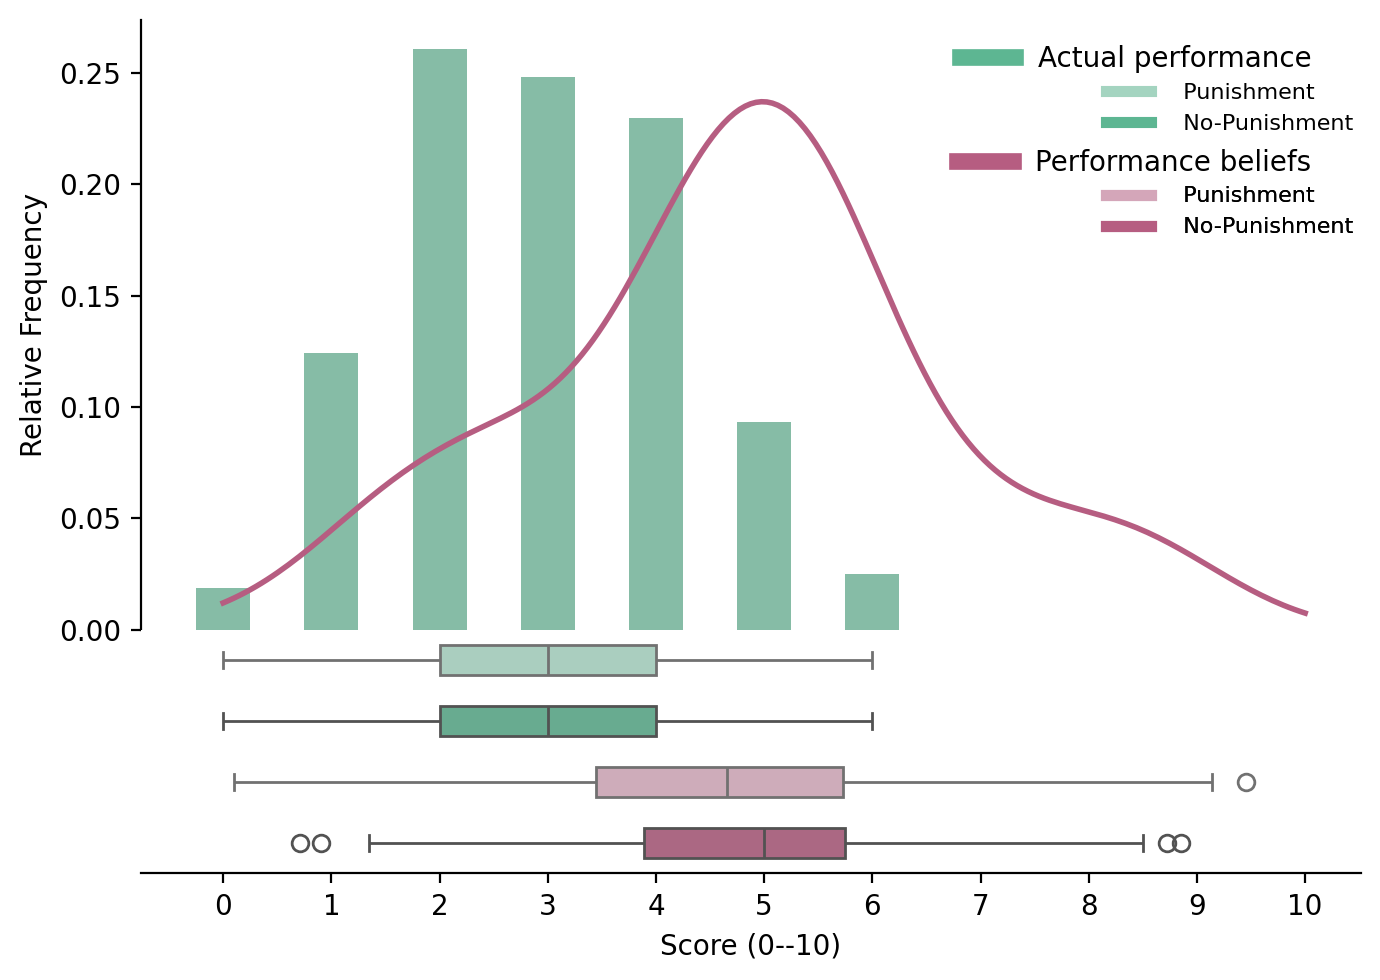
\includegraphics[width=0.75\linewidth]{figures/performance.png}
    \label{fig:performance}
    \begin{minipage}{0.85\linewidth}
    \footnotesize
    \textit{Note:} Distribution of correct predictions (within $10$~lbs of the true weight) over the first ten task rounds, by condition. Average performance is $2.93$ correct out of ten and is statistically indistinguishable across conditions.
    \end{minipage}
\end{figure}

\paragraph{(M3) Process ownership of the outcome.} A third mechanism, suggested by the heterogeneity of the delegation decision with respect to Player~A's performance documented in Result~1 above (and Column~(3) of Table~\ref{tab:del_decision_determinants}), is that Player~As who have a higher subjective probability of producing the high payoff for Player~B prefer to bring about that good outcome themselves rather than via the algorithm. The intuition draws on the psychological-ownership literature: people derive utility from being the proximate cause of a good outcome for another, and this utility is asymmetric with respect to outcomes \citep{steffel_passing_2016}. The data are consistent with this mechanism, but the supporting evidence is thin. The negative relationship between performance and delegation in the \textit{Punishment} condition is what process-ownership predicts: better-performing Player~As, who are more likely to deliver the high payoff, prefer to do so personally. The absence of this relationship in the \textit{No-Punishment} condition is consistent with process ownership being amplified by the moral salience that the punishment possibility introduces. We are explicit, however, that the supporting evidence consists of a single heterogeneity pattern in a 60-subject sub-sample and a comparison of selected non-delegator success rates; the pattern is the most consistent reading of the data we have, but not a confirmed mechanism. A direct test would require a treatment that varies process ownership while holding the punishment possibility fixed---for example, an arm in which the algorithm is presented as Player~A's own ``tool'' rather than as a separate agent.

\paragraph{(M4) Experimenter demand.} A final possibility is that the punishment possibility cues Player~A to behave more conservatively---for instance, to avoid an action (delegation) that the experimental setting itself implicitly frames as morally questionable. We cannot rule this mechanism out with our data. The most we can say is that two implications of a strong demand story are not borne out: if demand were dominant, Player~A's behavior should track elicited beliefs more tightly than it does, and the sharp performance heterogeneity in the \textit{Punishment} condition (better performers delegating less) would be hard to explain. Neither absence is decisive against the demand reading. We discuss the implications, and the design moves that would identify demand directly, in Section~\ref{conclusion}.

\medskip

In sum: M1 (anticipated differential punishment) is inconsistent with the data. M2 (effort to outperform the algorithm) is inconsistent with the data in its simple form. M3 (process ownership) is consistent with the data but supported only by exploratory heterogeneity analysis. M4 (experimenter demand) cannot be separated from M3 with the present design. The most economical reading---the one we adopt with explicit hedges in the Conclusion---is that the morally charged context introduced by the punishment possibility makes Player~A want to be the proximate cause of any good outcome for Player~B, while we acknowledge that an experimenter-demand story can produce qualitatively similar patterns. Disentangling the two is the cleanest direction for follow-up work.


\section{Discussion and Conclusion} \label{conclusion}

This paper asks two questions about how the prospect of punishment interacts with the use of algorithms as decision aids. Can decision-makers shift responsibility for bad outcomes onto algorithms by delegating their decisions? And does the anticipation of being held responsible motivate delegation in the first place? We address both questions in a preregistered online experiment in which Player~A makes a payoff-relevant prediction for Player~B and may delegate the prediction to an algorithm calibrated to perform as well as Player~A herself. A between-subject manipulation switches off punishment by Player~B in the \textit{No-Punishment} condition; the \textit{Punishment} preserves the natural setting in which the prospect of punishment is on the table.

Two findings emerge. First, and most striking, the \textit{prospect} of punishment \textit{reduces}, rather than increases, the propensity to delegate to the algorithm: $42.5\%$ of Player~As delegate when punishment is possible, compared to $59.3\%$ when it is not. This direction is the opposite of what the responsibility-avoidance literature would predict, and we view the reversal as the paper's main empirical contribution---noting that, because the result reverses the preregistered direction, the analyses we use to interpret it (Section~\ref{sec:mechanism}) are exploratory rather than confirmatory. Second, conditional on the outcome for Player~B, we cannot reject the hypothesis that delegated and self-made decisions are punished equally. The point estimate runs in the predicted direction (lower punishment under delegation in the bad-outcome cell) but is small relative to the test's confidence interval at the achieved sample size; we therefore frame Result~2 as a failure to detect insulation rather than as positive evidence that delegation cannot insulate. Player~A does not appear to be able to use this particular algorithm as a meaningful blame shield in the bounded sense the test can assess.

\paragraph{Mechanism.} Why does punishment reduce, rather than increase, delegation? The data are inconsistent with a simple anticipation mechanism: Player~As do not on average expect harsher punishment for delegated decisions, and they correctly anticipate the absence of differential punishment that we observe in Player~B's actual choices. The data are likewise inconsistent with the simple form of an effort story in which the prospect of punishment motivates Player~A to outperform the algorithm: among non-delegators, those in the \textit{No-Punishment} condition (where punishment is impossible) outperform those in the \textit{Punishment} condition, the reverse of what such a story implies. The reading most consistent with the data is one of \textit{process ownership}: Player~As who actively choose not to delegate take responsibility for the outcome, exert correspondingly higher effort, and that share is higher when punishment is on the table. The supporting evidence is exploratory rather than confirmatory, however, and rests on a single performance-by-delegation heterogeneity pattern in a 60-subject sub-sample (Column (3) of Table~\ref{tab:del_decision_determinants}); we cannot, with this design, separate process ownership cleanly from an experimenter-demand reading in which the punishment cue itself nudges Player~A toward direct engagement. We therefore present process ownership as the most consistent reading of the data we have, not as a confirmed mechanism. Disentangling it from demand is a clean direction for follow-up work, sketched below.

This refinement is consistent with, but goes beyond, the standard reading of the responsibility-avoidance literature. The classic finding---that delegation reduces punishment of the principal and that this prospect motivates delegation---was established in dictator-game settings where the underlying choice is between a known fair and a known unfair allocation, the intermediary is human, and the principal can be held accountable specifically for choosing a particular intermediary~\citep{bartling_shifting_2012,coffman_intermediation_2011,oexl_shifting_2013}. When the intermediary is an algorithm calibrated to mimic the principal and the underlying decision involves genuine uncertainty, none of the standard mechanisms through which delegation can shift responsibility---signal value of the delegation choice, the human-human punishment channel, the certainty of the unfair outcome---are available. What remains is a baseline outcome-based punishment, supplemented by an asymmetric desire to be the proximate cause of good outcomes when the moral stakes are salient.

\paragraph{Implications, with explicit bounds.} Our findings speak to the design of accountability regimes governing algorithmic decision-making. The European Union's AI~Act~\citep{european_union_ai_act_2024} and analogous regulatory frameworks elsewhere place increasing emphasis on assigning responsibility to human users of high-risk algorithmic systems. The implicit theory of behaviour underlying these provisions is that holding humans accountable for algorithm-mediated decisions \textit{disciplines} their use of those algorithms. Our results offer a behavioural complement to this view: when punishment is on the table, decision-makers in our setting do not simply delegate-and-blame the algorithm; they choose to take direct responsibility for the decision more often. From the perspective of efficiency, this need not be welfare-increasing: in domains where algorithms genuinely outperform humans, holding humans liable for outcomes may push decision-makers away from the more accurate technology. The trade-off between encouraging algorithmic adoption and assigning meaningful responsibility is, on this reading, sharper than the existing literature has suggested.

We note explicitly the bounds of this reading. Our evidence is a single online experiment with $322$ UK Prolific participants on a stylised weight-prediction task, with stakes of $\pounds 5$ for Player~B and a punishment range of $\pounds 0$--$\pounds 2$. The high-stakes algorithmic domains that motivate the regulatory debate---medical diagnosis, judicial risk assessment, hiring, credit allocation---differ from our setting in stake magnitude, professional context, expert training, the institutional structure of accountability, and the kind of population at the decision margin. We therefore view the result as identifying a behavioural channel that exists in principle and is detectable in our setting, not as a calibration of how big a lever accountability is in any specific applied domain. Mapping the magnitude of the effect against external benchmarks---e.g., physician adoption of diagnostic algorithms under malpractice exposure, or loan-officer deviation from credit-scoring algorithms under fair-lending audit---would require either domain-specific replication or instruments to which we do not have access. We flag this gap explicitly so that readers can calibrate the policy implication appropriately.

\paragraph{Limitations.} Several caveats are in order. The belief measure we elicit is unincentivised and noisy; it conveys ordinal patterns reliably but cannot support fine-grained quantitative claims about Player~A's anticipations. Two of the four belief scenarios are hypothetical conditional on the delegation decision, and all four are hypothetical in the \textit{No-Punishment} condition; this further limits the inference, and we plan to report the H2 patterns separately for the payoff-relevant and the hypothetical cells once the analysis pipeline is in place. We use the strategy method for Player~B's punishment decision, which is standard in this literature but may yield different absolute levels of punishment than a direct elicitation. Player~A also makes the eleventh prediction whether or not she ultimately decides to delegate, which equates the time cost of the two options but may signal her commitment differently than a design in which the prediction is skipped under delegation. We did not include a separate manipulation-comprehension check verifying that Player~A internalised the punishment-on/off distinction; we relied on the prominent screen-level framing and on attention-check pass rates as indirect evidence, but a future replication should add this check. The absolute stakes are modest (£5 high payoff, £0--2 punishment range): we cannot speak to how the effect scales with stakes, and a stake-magnitude robustness check is the first item in the future-research list below. Our sample is drawn from UK Prolific participants, which limits external validity along the dimensions in which Prolific samples differ from broader populations and from professional decision-makers in the high-stakes algorithmic domains we discuss above.

A natural concern is whether the punishment possibility cues Player~A to behave more conservatively for reasons unrelated to the substantive question---an experimenter-demand effect. We cannot rule this concern out from the data. The direction of any such effect is also ambiguous: a decision-maker who is reminded of being judged could plausibly delegate \textit{more} (to shed responsibility) or \textit{less} (to demonstrate effort and commitment); the literature does not unambiguously favour one over the other. We note two patterns weakly inconsistent with a strong demand reading---behaviour does not track elicited beliefs as tightly as a pure-demand story would predict, and the sharp performance heterogeneity in the \textit{Punishment} condition (better performers delegating less) is harder to motivate from demand alone---but we treat these as suggestive rather than dispositive. A direct test in the spirit of \citet{de_quidt_measuring_2018} would be the natural next step.

\paragraph{Directions for future research.} Several extensions would strengthen the inference. A direct-method companion would test the robustness of Result~2 against the strategy-method elicitation, and a meaningfully larger sample would let us put a tight confidence interval on the small but persistent point estimate of insulation under delegation. A condition in which Player~A is told explicitly that Player~B is unaware of the equal-performance calibration would test whether the relative-performance signal is the binding margin distinguishing our results from \citet{feier_hiding_2022}. Conditions that experimentally vary the algorithm's performance relative to Player~A (above, equal, below) would map the generality of the process-ownership reading. A demand-effect probe along the lines of \citet{de_quidt_measuring_2018} would put a credible upper bound on the contribution of M4. A stake-magnitude robustness check, varying the £5/£1 high/low payoffs and the £0--£2 punishment range, would speak to whether the effect scales with stakes in the direction that policy-relevant settings would imply. Finally, replication in a different country, in a different decision domain (e.g., a medical-triage or hiring vignette), or with a sample of professional decision-makers rather than online crowd-workers would speak directly to the external-validity bounds we describe above.

Taken together, our results suggest a more textured story than the one that has emerged from the existing literature on responsibility avoidance and algorithm aversion. Within the bounds of the setting we study, the capacity to use algorithms as a tool for shifting responsibility appears limited, and the prospect of being held responsible---rather than encouraging delegation as a hedge---appears to push decision-makers towards direct engagement with the consequential choice. Whether the same channel operates in the high-stakes algorithmic domains that animate the regulatory debate is an empirical question that this study can frame but cannot, on its own, answer.


\pagebreak

\bibliographystyle{aer}
\bibliography{ProjectAlgorithm}
\newpage{}

\setcounter{page}{1}
\renewcommand{\thepage}{A-\arabic{page}}

\section*{Appendix} \label{appendix}

\appendix

\section{Additional Tables} \label{appendix:tables}

\subsection{Condition balance --- Player A} \label{appendix:sum_stats}

\begin{table}[!htbp]
    \centering
    \caption{Condition balance --- Player~A}
    \label{tab:treatment_balance}
    \begin{tabular}{l|rrr}
                  Variable &  \textit{Punishment} &  \textit{No-Punishment} &  $p$-value \\ \hline
                           Age &  $39.026$ &  $37.877$ &  $0.552$ \\
                        Female &  $0.487$ &  $0.494$ &  $1.000$ \\
         Socio-economic status &  $5.179$ &  $5.321$ &  $0.564$ \\
                   Went to uni &  $0.575$ &  $0.556$ &  $0.928$ \\
              Technology score &  $2.087$ &  $2.284$ &  $0.322$ \\
           Leadership position &  $0.362$ &  $0.333$ &  $0.824$ \\
    \end{tabular}
    \begin{minipage}{0.95\textwidth}\footnotesize
    \textit{Note:} Mean values by condition for Player~A, with $p$-values from two-sided $t$-tests for continuous variables and Chi-squared tests for binary variables. \textit{Socio-economic status} is self-reported on a $1$--$10$ scale. \textit{Went to uni} indicates a university degree. \textit{Technology score} is constructed from weekly device usage, programming skills, cryptocurrency knowledge, technology use at work, and similar items. \textit{Leadership position} indicates self-reported management or supervisory experience.
    \end{minipage}
\end{table}


\subsection{Condition balance --- Player B} \label{appendix:sum_stats_B}

\begin{table}[!htbp]
    \centering
    \caption{Condition balance --- Player~B}
    \label{tab:treatment_balance_B}
    \begin{tabular}{l|rrr}
                  Variable &  \textit{Punishment} &  \textit{No-Punishment} &  $p$-value \\ \hline
                           Age &  $37.087$ &  $42.356$ &  $0.011$ \\
                        Female &  $0.588$ &  $0.493$ &  $0.314$ \\
         Socio-economic status &  $5.425$ &  $5.110$ &  $0.204$ \\
                   Went to uni &  $0.688$ &  $0.481$ &  $0.013$ \\
              Technology score &  $1.363$ &  $1.333$ &  $0.869$ \\
           Leadership position &  $0.287$ &  $0.321$ &  $0.771$ \\
    \end{tabular}
    \begin{minipage}{0.95\textwidth}\footnotesize
    \textit{Note:} Mean values by condition for Player~B, with $p$-values from two-sided $t$-tests for continuous variables and Chi-squared tests for binary variables. \textit{Socio-economic status} is self-reported on a $1$--$10$ scale; \textit{Went to uni} indicates a university degree; \textit{Technology score} is constructed from weekly device usage, programming skills, cryptocurrency knowledge, technology use at work, and similar items; \textit{Leadership position} indicates self-reported management or supervisory experience.
    \end{minipage}
\end{table}


\subsection{Full regression results --- delegation decision} \label{appendix:regs}

\begin{table}[!htbp]
\centering
\caption{Determinants of the delegation decision --- full controls}
\label{tab:reg_delegation}
\begin{tabular}{@{\extracolsep{5pt}}lcc|c}
\\[-1.8ex]\hline
\hline \\[-1.8ex]
& \multicolumn{3}{c}{Dependent variable: \textit{Delegation}}\\[0.1cm]
& \multicolumn{2}{c}{\textit{Full sample}} & \textit{Punishment only} \\
\\[-1.8ex] & (1) & (2) & (3) \\
\hline \\[-1.8ex]
 No-Punishment indicator & $0.677$ & $0.757$ &  \\
  & $(0.320)$ & $(0.334)$ &  \\[0.1cm]
 Punishment beliefs: bad outcome &  &  & $0.937$ \\
  &  &  & $(0.751)$ \\[0.1cm]
 Punishment beliefs: good outcome &  &  & $1.579$ \\
  &  &  & $(0.741)$ \\[0.1cm]
 Task performance &  & $-0.192$ & $-0.609$ \\
  &  & $(0.128)$ & $(0.236)$ \\[0.1cm]
 Age &  & $-0.004$ & $0.064$ \\
  &  & $(0.015)$ & $(0.030)$ \\[0.1cm]
 Female &  & $0.350$ & $1.334$ \\
  &  & $(0.369)$ & $(0.793)$ \\[0.1cm]
 Socio-economic status &  & $-0.058$ & $-0.003$ \\
  &  & $(0.116)$ & $(0.219)$ \\[0.1cm]
 Went to uni &  & $0.091$ & $-0.433$ \\
  &  & $(0.364)$ & $(0.707)$ \\[0.1cm]
 Technology score &  & $-0.078$ & $0.059$ \\
  &  & $(0.153)$ & $(0.283)$ \\[0.1cm]
 Leadership position &  & $0.676$ & $-0.387$ \\
  &  & $(0.367)$ & $(0.729)$ \\[0.1cm]
 Constant & $-0.302$ & $0.402$ & $-1.842$ \\
  & $(0.226)$ & $(0.930)$ & $(2.103)$ \\[0.1cm]
\hline \\[-1.8ex]
 N & $161$ & $159$ & $60$ \\
 Pseudo $R^2$ & $0.020$ & $0.049$ & $0.246$ \\
\hline
\hline \\[-1.8ex]
\multicolumn{4}{p{0.85\textwidth}}{\footnotesize \textit{Note:} Logit estimates with robust (HC1) standard errors in parentheses. Two subjects in Column~(2) are dropped due to missing socio-demographic data. Column~(3) restricts to the \textit{Punishment} condition and excludes subjects who failed the attention check on the belief-elicitation screen, as preregistered. The belief variables in Column~(3) are within-subject differences in expected punishment between non-delegated and delegated decisions for each outcome. Following AEA editorial policy, significance stars are not reported in the table.}
\end{tabular}
\end{table}


\subsection{Robustness --- delegation decision} \label{appendix:reg_delegation_robustness}

\begin{table}[!htbp]
\centering
\scriptsize
\caption{Determinants of the delegation decision --- robustness}
\label{tab:reg_delegation_robustness}
\begin{tabular}{@{\extracolsep{5pt}}lcc|c}
\\[-1.8ex]\hline
\hline \\[-1.8ex]
& \multicolumn{3}{c}{Dependent variable: \textit{Delegation}}\\[0.1cm]
& \multicolumn{2}{c}{\textit{Full sample}} & \textit{Punishment} (no excl.) \\
\\[-1.8ex] & (1) & (2) & (3) \\
\hline \\[-1.8ex]
 Punishment indicator & $-0.771$ & $-0.677$ &  \\
  & $(0.336)$ & $(0.320)$ &  \\[0.1cm]
 Task performance & $-0.277$ &  & $-0.395$ \\
  & $(0.149)$ &  & $(0.185)$ \\[0.1cm]
 Overconfidence & $-0.103$ &  &  \\
  & $(0.094)$ &  &  \\[0.1cm]
 Punishment beliefs: bad outcome (no del.~$-$~del.) &  &  & $-0.277$ \\
  &  &  & $(0.499)$ \\[0.1cm]
 Punishment beliefs: good outcome (no del.~$-$~del.) &  &  & $0.812$ \\
  &  &  & $(0.529)$ \\[0.1cm]
\hline \\[-1.8ex]
 Controls & yes & no & yes \\
 Attention-check excl. & yes (Player A) & n/a & no \\
 Sample & Full & Full & Punishment \\
 N & $159$ & $161$ & $78$ \\
 Pseudo $R^2$ & $0.055$ & $0.020$ & $0.114$ \\
\hline
\hline \\[-1.8ex]
\multicolumn{4}{p{0.85\textwidth}}{\footnotesize \textit{Note:} Robustness specifications for the delegation logit. Column (1) adds \textit{overconfidence} (defined as the weighted-average belief about own performance minus actual performance) to the main full-sample specification. The treatment effect remains: \textit{Punishment indicator} $p=0.022$. \textit{Overconfidence} is not significantly associated with delegation $p=0.272$. Column (2) reproduces the unconditional treatment effect for completeness ($p=0.034$; identical to the main Col (1)). Column (3) restricts to the \textit{Punishment} condition and includes the within-subject belief differences but \textit{does not} exclude subjects who failed the belief-screen attention check; the heterogeneity result is preserved: \textit{Task performance} $p=0.033$; \textit{Punishment beliefs: good outcome} $p=0.125$. Robust HC1 standard errors in parentheses. Following AEA editorial policy, significance stars are not reported in the table.}
\end{tabular}
\end{table}


\subsection{Determinants of Player~B's chosen punishment} \label{appendix:reg_punishment}

\begin{table}[!htbp]
\centering
\caption{Determinants of Player~B's chosen punishment}
\label{tab:reg_punishment}
\begin{tabular}{@{\extracolsep{5pt}}lccc|ccc}
\\[-1.8ex]\hline
\hline \\[-1.8ex]
& \multicolumn{6}{c}{Dependent variable: \textit{Punishment}}\\[0.1cm]
& \multicolumn{3}{c}{\textit{Full sample}} & \multicolumn{3}{c}{\textit{Passers}} \\
& \textit{Level} (\pounds) & \multicolumn{2}{c}{\textit{Difference} (\pounds)} & \textit{Level} (\pounds) & \multicolumn{2}{c}{\textit{Difference} (\pounds)} \\
\\[-1.8ex] & (1) & (2) & (3) & (4) & (5) & (6) \\
\hline \\[-1.8ex]
 Delegated & $0.032$ &  &  & $0.001$ &  &  \\
  & $(0.052)$ &  &  & $(0.054)$ &  &  \\[0.1cm]
 Bad outcome & $0.256^{***}$ & $0.103^{*}$ & $0.103^{*}$ & $0.260^{***}$ & $0.078$ & $0.078$ \\
  & $(0.071)$ & $(0.057)$ & $(0.059)$ & $(0.080)$ & $(0.052)$ & $(0.053)$ \\[0.1cm]
 Delegated $\times$ Bad outcome & $-0.103^{*}$ &  &  & $-0.078$ &  &  \\
  & $(0.058)$ &  &  & $(0.052)$ &  &  \\[0.1cm]
 Player B belief about Player A perf. & $-0.020$ &  & $-0.006$ & $0.001$ &  & $-0.006$ \\
  & $(0.032)$ &  & $(0.029)$ & $(0.037)$ &  & $(0.038)$ \\[0.1cm]
 Age & $0.002$ &  & $-0.009^{**}$ & $-0.001$ &  & $-0.009^{**}$ \\
  & $(0.005)$ &  & $(0.003)$ & $(0.006)$ &  & $(0.004)$ \\[0.1cm]
 Female & $-0.100$ &  & $-0.012$ & $-0.064$ &  & $0.003$ \\
  & $(0.128)$ &  & $(0.109)$ & $(0.140)$ &  & $(0.132)$ \\[0.1cm]
 Socio-economic status & $0.083^{*}$ &  & $0.029$ & $0.072$ &  & $0.041$ \\
  & $(0.047)$ &  & $(0.024)$ & $(0.049)$ &  & $(0.028)$ \\[0.1cm]
 Went to uni & $-0.196$ &  & $0.051$ & $-0.098$ &  & $0.023$ \\
  & $(0.140)$ &  & $(0.070)$ & $(0.142)$ &  & $(0.075)$ \\[0.1cm]
 Technology score & $0.073$ &  & $-0.022$ & $0.030$ &  & $-0.012$ \\
  & $(0.053)$ &  & $(0.027)$ & $(0.059)$ &  & $(0.033)$ \\[0.1cm]
 Leadership position & $0.083$ &  & $0.143$ & $0.061$ &  & $0.174$ \\
  & $(0.142)$ &  & $(0.122)$ & $(0.164)$ &  & $(0.145)$ \\[0.1cm]
 Constant & $-0.077$ & $-0.032$ & $0.116$ & $0.020$ & $-0.001$ & $0.076$ \\
  & $(0.328)$ & $(0.051)$ & $(0.320)$ & $(0.374)$ & $(0.053)$ & $(0.397)$ \\[0.1cm]
\hline \\[-1.8ex]
 Observations & $320$ & $160$ & $160$ & $268$ & $134$ & $134$ \\
 Subjects & $80$ & $80$ & $80$ & $67$ & $67$ & $67$ \\
 Adj.\ $R^2$ & $0.077$ & $0.008$ & $0.038$ & $0.030$ & $0.001$ & $0.043$ \\
\hline
\hline \\[-1.8ex]
\multicolumn{7}{p{0.85\textwidth}}{\footnotesize \textit{Note:} Columns~(1) and~(4): OLS regression of Player~B's chosen punishment level on a delegation indicator, a bad-outcome indicator, their interaction, Player~B's belief about Player~A's performance, and a vector of socio-demographic controls; sample stacked over the four (delegation, outcome) cells of the strategy method (4 observations per Player~B). Columns~(2)/(5) and~(3)/(6): OLS regression of the within-subject delegation insulation (\textit{punish\_nodel} $-$ \textit{punish\_del}) on a bad-outcome indicator and, in Columns~(3)/(6), additional controls; sample stacked over the two outcome cells (2 observations per Player~B). In the difference specifications, the intercept is the average insulation in the good-outcome cell and the bad-outcome coefficient is the additional insulation in the bad-outcome cell. Columns~(1)--(3) use the full Punishment-condition sample. Columns~(4)--(6) restrict to Player~Bs who passed the attention check on the punishment-elicitation screen, as preregistered. Standard errors clustered at the Player~B level. Significance: $^{*}\,p<0.10$; $^{**}\,p<0.05$; $^{***}\,p<0.01$ (two-sided).}
\end{tabular}
\end{table}


\subsection{Robustness --- Player~B's chosen punishment} \label{appendix:reg_punishment_robustness}

\begin{table}[!htbp]
\centering
\caption{Determinants of Player~B's chosen punishment --- robustness}
\label{tab:reg_punishment_robustness}
\begin{tabular}{lcc}
\\[-1.8ex]\hline
\hline \\[-1.8ex]
& \multicolumn{2}{c}{Dependent variable: \textit{Punishment}}\\[0.1cm]
& \textit{Excl.} & \textit{Incl. att.\ failers} \\
\\[-1.8ex] & (1) & (2) \\
\hline \\[-1.8ex]
 Delegated & $0.001$ & $0.032$ \\
  & $(0.054)$ & $(0.052)$ \\[0.1cm]
 Bad outcome & $0.260$ & $0.256$ \\
  & $(0.080)$ & $(0.071)$ \\[0.1cm]
 Delegated $\times$ Bad outcome & $-0.078$ & $-0.103$ \\
  & $(0.052)$ & $(0.058)$ \\[0.1cm]
 Player B belief about Player A perf. (wa) & $0.001$ & $-0.020$ \\
  & $(0.037)$ & $(0.032)$ \\[0.1cm]
 Age & $-0.001$ & $0.002$ \\
  & $(0.006)$ & $(0.005)$ \\[0.1cm]
 Female & $-0.064$ & $-0.100$ \\
  & $(0.140)$ & $(0.128)$ \\[0.1cm]
 Socio-economic status & $0.072$ & $0.083$ \\
  & $(0.049)$ & $(0.047)$ \\[0.1cm]
 Went to uni & $-0.098$ & $-0.196$ \\
  & $(0.142)$ & $(0.140)$ \\[0.1cm]
 Technology score & $0.030$ & $0.073$ \\
  & $(0.059)$ & $(0.053)$ \\[0.1cm]
 Leadership position & $0.061$ & $0.083$ \\
  & $(0.164)$ & $(0.142)$ \\[0.1cm]
 Constant & $0.020$ & $-0.077$ \\
  & $(0.374)$ & $(0.328)$ \\[0.1cm]
\hline \\[-1.8ex]
 Attention-check excl. & yes & no \\
 N (subject-by-cell) & $268$ & $320$ \\
 Adj.\ $R^2$ & $0.030$ & $0.077$ \\
\hline
\hline \\[-1.8ex]
\multicolumn{3}{p{0.85\textwidth}}{\footnotesize \textit{Note:} Punishment regression with Player~B's belief about Player~A's performance (\textit{wa\_difficulty}) added as a regressor. Column (1) excludes Player~Bs who failed the punishment-screen attention check (preregistered); Column (2) keeps them. Standard errors clustered at the Player~B level. The delegation, outcome, and interaction coefficients are stable across both specifications, and the belief regressor is not significantly associated with chosen punishment. H2 paired-test on the bad-outcome cell: with exclusion paired-$t$ $p=0.153$, Wilcoxon $p=0.533$ ($n=67$); without exclusion paired-$t$ $p=0.131$, Wilcoxon $p=0.544$ ($n=80$). Following AEA editorial policy, significance stars are not reported.}
\end{tabular}
\end{table}


\section{Preregistration and deviations} \label{appendix:pap}

The experiment was preregistered prior to data collection. The preregistration document specifies the two hypotheses (H1 and H2 in the body), the sample-size target ($80$ subjects per role per condition, motivated by an ex-ante power calculation reproduced in the registry), the randomisation procedure, the attention-check exclusion rule, and the test direction for each preregistered comparison.

For full transparency, the table below summarises every analysis reported in the body of the paper, the corresponding preregistered specification, and any deviation. We treat the H1 reversal in Section~\ref{sec:result1} as a confirmatory test of the preregistered direction (which it rejects), and all subsequent mechanism analyses (Section~\ref{sec:mechanism}) as exploratory.

\begin{table}[!htbp]
\centering
\caption{Preregistered tests, reported tests, and deviations}
\label{tab:pap_deviations}
\begin{tabular}{p{0.32\textwidth}|p{0.32\textwidth}|p{0.30\textwidth}}
\hline
\hline
Preregistered specification & As reported & Deviation / rationale \\ \hline
H1: between-subject test of \textit{Punishment} vs \textit{No-Punishment} delegation rates; one-sided in the H1 direction (more delegation under \textit{Punishment}) & Two-sided Chi-squared and Fisher's exact, $p=0.049$ / $0.041$ & Direction reversed; one-sided test in H1 direction is non-significant by construction. We report two-sided to be transparent about what the data show. \\[0.3cm]
H2: paired test of Player~B punishment in the bad-outcome cell, delegated vs non-delegated, attention-check passers only & Paired $t$-test, $p=0.153$; Wilcoxon signed-rank, $p=0.533$ & As preregistered. \\[0.3cm]
Logit of delegation on condition + controls (Table~\ref{tab:del_decision_determinants}, Cols (1)--(2)) & As reported & As preregistered. \\[0.3cm]
Logit on \textit{Punishment} sub-sample with belief differences (Col (3)) & As reported & Specification preregistered; sample restriction follows the preregistered attention-check rule. \\[0.3cm]
Mechanism analyses M1--M4 (Section~\ref{sec:mechanism}) & As reported & \textit{Not preregistered.} Treated as exploratory throughout. \\[0.3cm]
Effort-comparison statistics among non-delegators (Section~\ref{sec:mechanism}, M2) & As reported & \textit{Not preregistered.} Treated as exploratory. \\
\hline
\hline
\multicolumn{3}{p{0.95\textwidth}}{\footnotesize \textit{Note:} The preregistration document is available at \textit{[registry link to be added at submission]}. The registry ID is \textit{[ID to be added at submission]}.}
\end{tabular}
\end{table}

\section{CONSORT-style flow diagram} \label{appendix:attrition}

A CONSORT-style flow diagram showing recruitment, attrition, attention-check exclusion, and final analysis sample size by condition and role is in preparation and will appear here once the analysis pipeline produces the underlying counts. The structure of the diagram is sketched below; cell counts pending.

\begin{figure}[!htbp]
\centering
\caption{Flow of participants through the experiment --- structure (counts pending)}
\label{fig:consort}
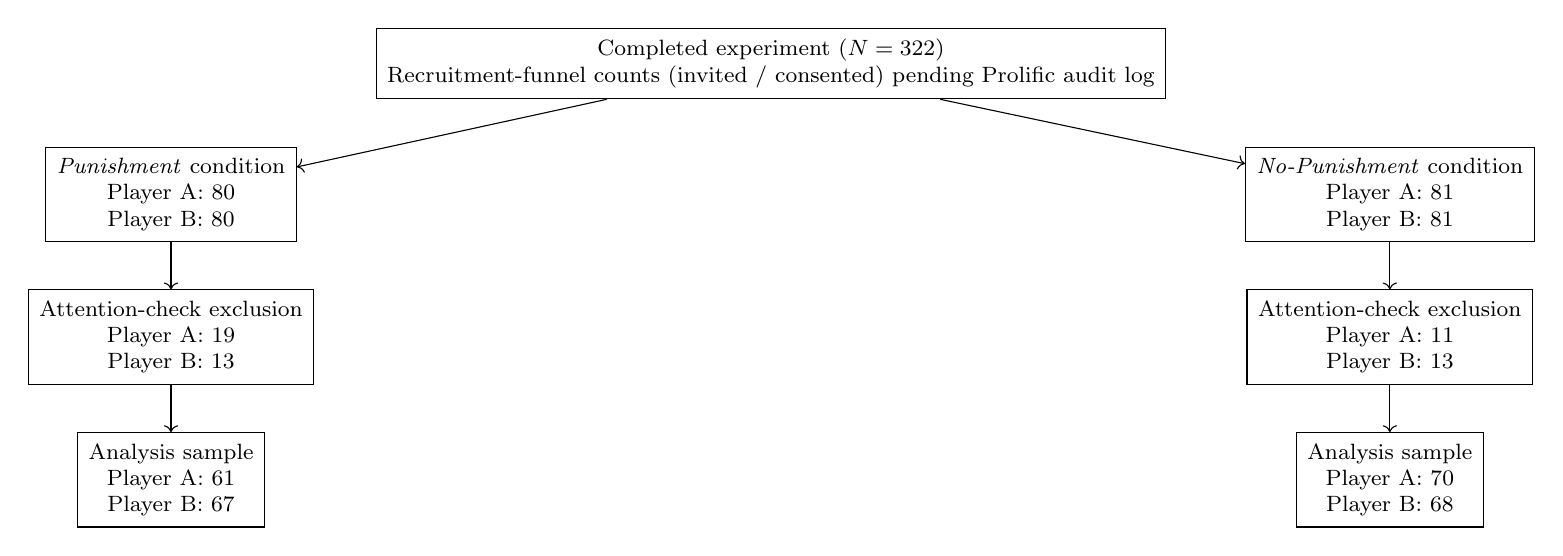
\begin{tikzpicture}[node distance=0.6cm and 0.6cm, every node/.style={draw, rectangle, align=center, font=\footnotesize, inner sep=4pt}]
\node (rand) {Completed experiment ($N=322$)\\Recruitment-funnel counts (invited / consented) pending Prolific audit log};
\node (pun) [below left=of rand, xshift=-0.4cm] {\textit{Punishment} condition\\Player A: $80$\\Player B: $80$};
\node (nopun) [below right=of rand, xshift=0.4cm] {\textit{No-Punishment} condition\\Player A: $81$\\Player B: $81$};
\node (att_p) [below=of pun] {Attention-check exclusion\\Player A: $19$\\Player B: $13$};
\node (att_np) [below=of nopun] {Attention-check exclusion\\Player A: $11$\\Player B: $13$};
\node (final_p) [below=of att_p] {Analysis sample\\Player A: $61$\\Player B: $67$};
\node (final_np) [below=of att_np] {Analysis sample\\Player A: $70$\\Player B: $68$};
\draw[->] (rand) -- (pun);
\draw[->] (rand) -- (nopun);
\draw[->] (pun) -- (att_p);
\draw[->] (nopun) -- (att_np);
\draw[->] (att_p) -- (final_p);
\draw[->] (att_np) -- (final_np);
\end{tikzpicture}
\end{figure}

\section{Additional Figures} \label{appendix:figures}

\subsection{Experimental timelines}

\begin{figure}[!htbp]
    \centering
    \caption{Experimental timeline --- Player A}
    \label{fig:design_playerA}
    \scalebox{0.85}{
    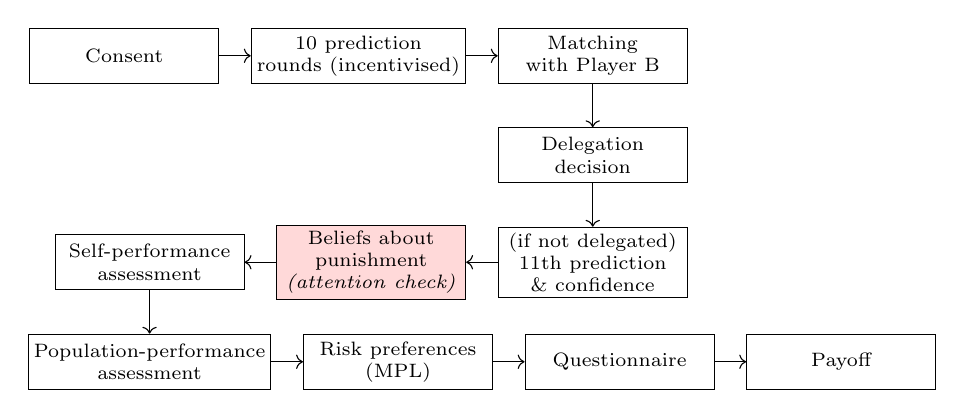
\begin{tikzpicture}[node distance=0.55cm and 0.4cm, every node/.style={draw, rectangle, align=center, font=\scriptsize, minimum width=2.4cm, minimum height=0.7cm, inner sep=2pt}, ac/.style={fill=red!15}]
    \node (consent) {Consent};
    \node (rounds) [right=of consent] {10 prediction\\rounds (incentivised)};
    \node (match) [right=of rounds] {Matching\\with Player B};
    \node (deleg) [below=of match] {Delegation\\decision};
    \node (predict) [below=of deleg] {(if not delegated)\\11th prediction\\\& confidence};
    \node (beliefs) [left=of predict, ac] {Beliefs about\\punishment\\\textit{(attention check)}};
    \node (selfperf) [left=of beliefs] {Self-performance\\assessment};
    \node (popperf) [below=of selfperf] {Population-performance\\assessment};
    \node (risk) [right=of popperf] {Risk preferences\\(MPL)};
    \node (qx) [right=of risk] {Questionnaire};
    \node (payoff) [right=of qx] {Payoff};
    \draw[->] (consent) -- (rounds);
    \draw[->] (rounds) -- (match);
    \draw[->] (match) -- (deleg);
    \draw[->] (deleg) -- (predict);
    \draw[->] (predict) -- (beliefs);
    \draw[->] (beliefs) -- (selfperf);
    \draw[->] (selfperf) -- (popperf);
    \draw[->] (popperf) -- (risk);
    \draw[->] (risk) -- (qx);
    \draw[->] (qx) -- (payoff);
    \end{tikzpicture}
    }
    \begin{minipage}{0.95\linewidth}
    \footnotesize
    \textit{Note:} Screen sequence presented to Player~A. The shaded screen carries the preregistered attention check used to identify subjects excluded from belief-related analyses. The 11th-prediction-and-confidence screen is skipped if Player~A delegates to the algorithm.
    \end{minipage}
\end{figure}

\begin{figure}[!htbp]
    \centering
    \caption{Experimental timeline --- Player B}
    \label{fig:design_playerB}
    \scalebox{0.85}{
    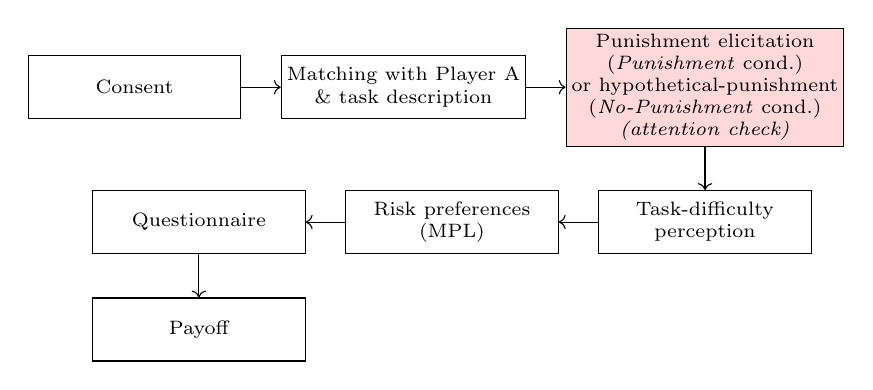
\begin{tikzpicture}[node distance=0.55cm and 0.5cm, every node/.style={draw, rectangle, align=center, font=\scriptsize, minimum width=2.7cm, minimum height=0.8cm, inner sep=2pt}, ac/.style={fill=red!15}]
    \node (consent) {Consent};
    \node (match) [right=of consent] {Matching with Player A\\\& task description};
    \node (pun) [right=of match, ac] {Punishment elicitation\\(\textit{Punishment} cond.)\\or hypothetical-punishment\\(\textit{No-Punishment} cond.)\\\textit{(attention check)}};
    \node (diff) [below=of pun] {Task-difficulty\\perception};
    \node (risk) [left=of diff] {Risk preferences\\(MPL)};
    \node (qx) [left=of risk] {Questionnaire};
    \node (payoff) [below=of qx] {Payoff};
    \draw[->] (consent) -- (match);
    \draw[->] (match) -- (pun);
    \draw[->] (pun) -- (diff);
    \draw[->] (diff) -- (risk);
    \draw[->] (risk) -- (qx);
    \draw[->] (qx) -- (payoff);
    \end{tikzpicture}
    }
    \begin{minipage}{0.95\linewidth}
    \footnotesize
    \textit{Note:} Screen sequence presented to Player~B. The shaded screen carries the preregistered attention check used to identify subjects excluded from punishment-related analyses. In the \textit{No-Punishment} condition, no actual punishment is implemented; the elicitation is hypothetical and serves to maintain comparability of the screen sequence across conditions.
    \end{minipage}
\end{figure}

\subsection{Punishment frequencies} \label{appendix:figs:punishment}

\begin{figure}[!htbp]
    \centering
    \caption{Frequencies of punishment and beliefs about punishment}
    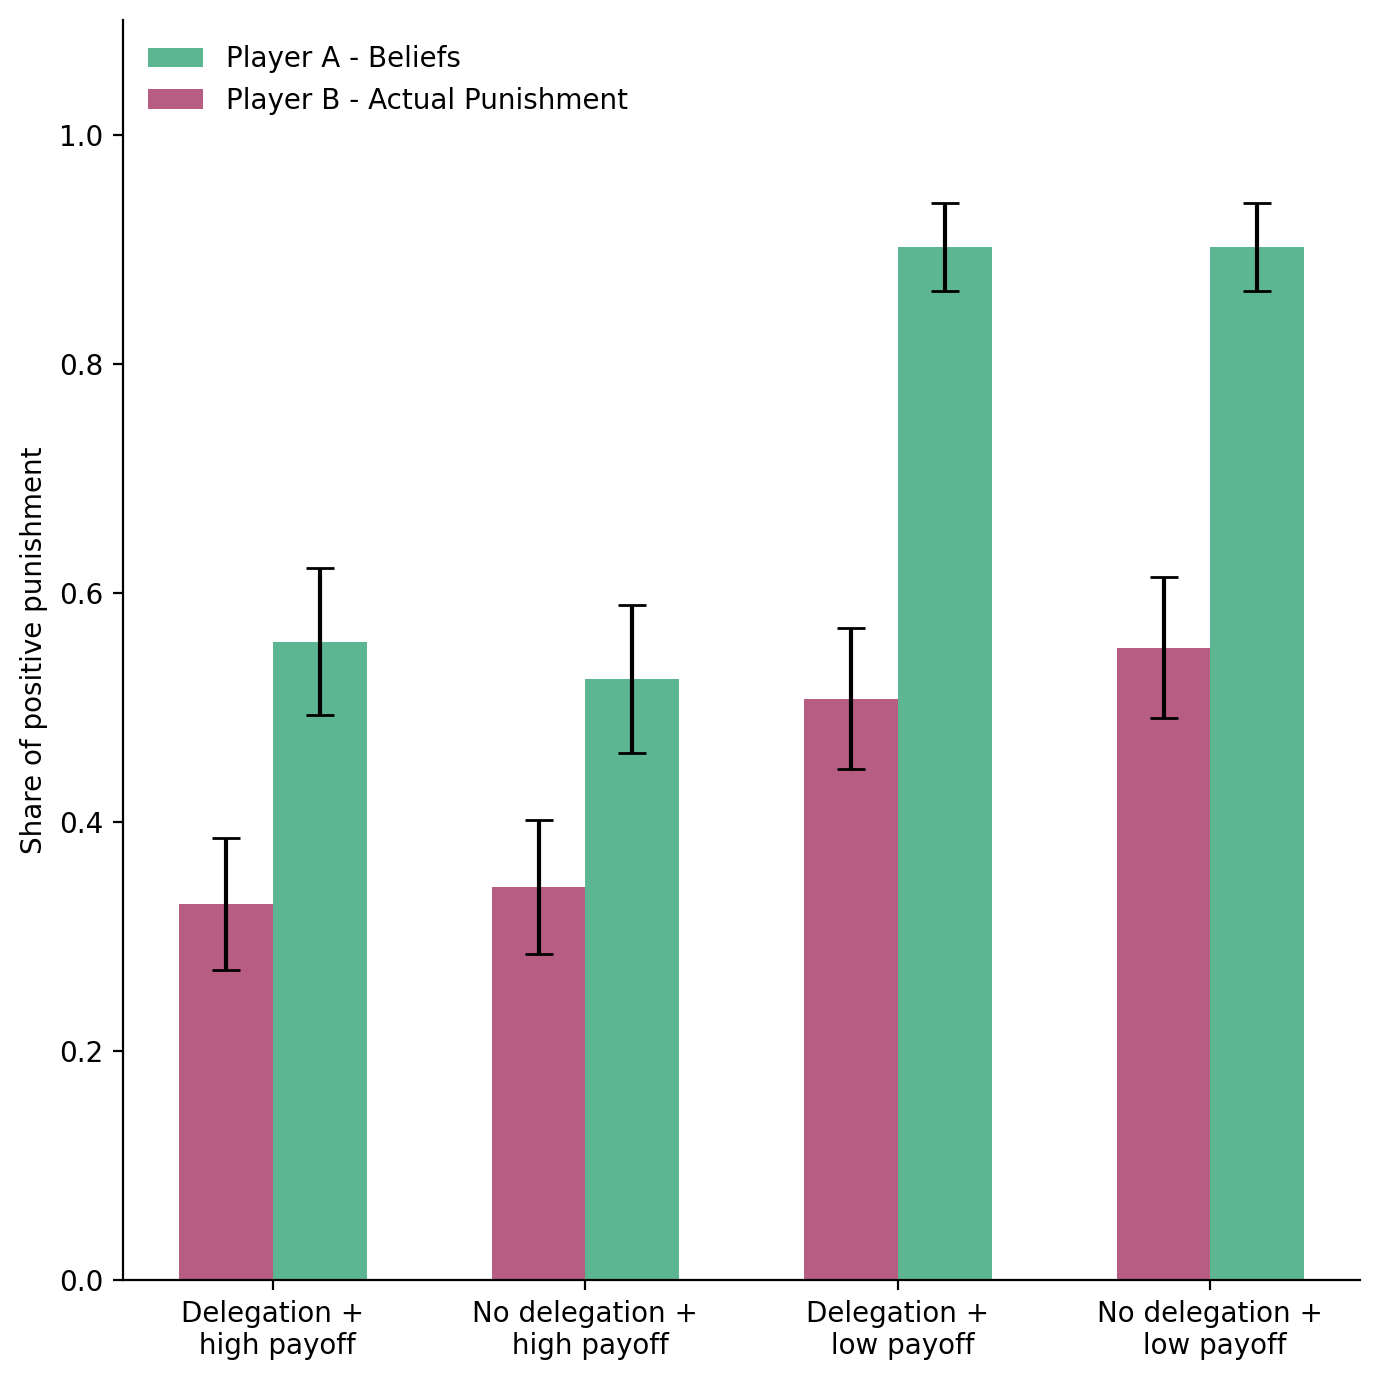
\includegraphics[width=0.6\linewidth]{figures/punishment_shares.png}
    \label{fig:punishment_frequencies}
    \begin{minipage}{0.85\linewidth}
    \footnotesize
    \textit{Note:} Share of Player~Bs choosing strictly positive punishment in each of the four scenarios (solid bars) and share of Player~As assigning a strictly positive expected punishment in each scenario (hollow bars).
    \end{minipage}
\end{figure}


\end{document}
